\documentclass[a4paper, 12pt]{article}
\usepackage[utf8x]{inputenc}
\usepackage[english, russian]{babel}
\usepackage[left=25mm, top=25mm, right=25mm, bottom=25mm]{geometry}
\usepackage{cmap}
\usepackage{indentfirst}
\usepackage{tikz}
\usepackage{float}
\usepackage{amsmath, amsfonts, amssymb}
\usepackage{graphicx}
\usepackage{hyperref}
\usepackage{listings}
\usepackage{caption}
\usepackage{subcaption}
\usepackage{xcolor}
\usepackage{etoolbox}
\usepackage{titlesec}
\pagestyle{plain}
\patchcmd{\tableofcontents}{\contentsname}{\centering\contentsname}{}{}
\titleformat{\section}[block]{\normalfont\large\bfseries\centering}{}{0pt}{}
\titleformat{\subsection}[block]{\normalfont\normalsize\bfseries\centering}{}{0pt}{}
\allowdisplaybreaks
\graphicspath{{src/images/}}
\usetikzlibrary{patterns}
\definecolor{LightGray}{gray}{0.95}
\definecolor{LightGray2}{gray}{0.7}
\lstdefinestyle{code}{
    language=MATLAB, % replace language here
    basicstyle=\footnotesize\ttfamily,
    % numbers=left,
    % numberstyle=\scriptsize\color{gray},
    % stepnumber=1,
    % numbersep=5pt,
    backgroundcolor=\color{LightGray},
    showspaces=false,
    showstringspaces=false,
    showtabs=false,
    tabsize=4,
    captionpos=b,
    breaklines=true,
    breakatwhitespace=false,
    frame=single,
    rulecolor=\color{LightGray2},
    linewidth=\linewidth,
    keywordstyle=\color{blue}\bfseries,
    commentstyle=\color{green!40!black},
    stringstyle=\color{purple},
    escapeinside={\%*}{*)},
    inputencoding=utf8x,
    xleftmargin=0pt,
    framexleftmargin=0pt,
    framexrightmargin=0pt
}
\lstset{style=code}
\hypersetup{
    colorlinks=true,
    linkcolor=blue,
    filecolor=magenta,
    urlcolor=cyan,
    pdftitle={contents setup},
    pdfpagemode=FullScreen,
}


\begin{document}
    \begin{titlepage}

        \begin{center}
        Федеральное государственное автономное образовательное учреждение высшего образования
        «Национальный Исследовательский Университет ИТМО»
        \vfill
        
        
\includegraphics[width=0.3\textwidth]{itmo.png} % requires /src/images/itmo.png

        {\large\bf ЛАБОРАТОРНАЯ РАБОТА №C}\\
        {\large\bf ПРЕДМЕТ «ТЕОРИЯ АВТОМАТИЧЕСКОГО УПРАВЛЕНИЯ»}\\
        {\large\bf ТЕМА «СЛЕЖЕНИЕ И КОМПЕНСАЦИЯ: ФРАНКИС, ДЭВИСОН И НАБЛЮДАТЕЛИ»}\\
        Вариант №2
        \vfill

        \begin{flushright}
            \begin{minipage}{.45\textwidth}
            {
                \hbox{Преподаватель:}
                \hbox{Пашенко А. В.}
                \hbox{}
                \hbox{Выполнил:}
                \hbox{Румянцев А. А.}
                \hbox{}
                \hbox{Факультет: СУиР}
                \hbox{Группа: R3341}
                \hbox{Поток: ТАУ R22 бак 1.1.1}
            }
            \end{minipage}
        \end{flushright}
        \vfill
  
        Санкт-Петербург\\
        2025
        \end{center}
    \end{titlepage}
    
    \tableofcontents

    \newpage
    \section{Задание 1. Слежение и компенсация: матричные уравнения}
    Рассмотрим систему
    \begin{align}
    \begin{cases}
        \dot{x}=Ax+Bu+B_ff,\\
        y=Cx+Du+D_ff,
    \end{cases}
    x(0)=\begin{bmatrix}
        0\\0\\0
    \end{bmatrix},\label{eq:sys1}
    \end{align}
    генератор внешнего возмущения
    \begin{align}
    \begin{cases}
        \dot{w}=\Gamma_f w_f,\\
        f=Y_fw_f,
    \end{cases} w_f(0)=\begin{bmatrix}
        1\\1\\1\\1\\
    \end{bmatrix}\label{eq:sys12}
    \end{align}
    и генератор задающего воздействия
    \begin{align}
    \begin{cases}
        \dot{w}_g=\Gamma_gw_g,\\
        g=Y_gw_g,
    \end{cases} w_g(0)\label{eq:sys13}
    \end{align}
    при параметрах объекта управления
    $$
    A=\begin{bmatrix}
        5 &2 &7\\
        2 &1 &2\\
        -2 &-3 &-4
    \end{bmatrix},\ B=\begin{bmatrix}
        3\\1\\-1
    \end{bmatrix},\ B_f=\begin{bmatrix}
        -4 &-1\\
        0 &0\\
        4 &0
    \end{bmatrix},\ C=\begin{bmatrix}
        2\\0\\3
    \end{bmatrix}^T,\ D=2,\ D_f=\begin{bmatrix}
        8\\3
    \end{bmatrix}^T
    $$
    и параметрах генератора
    $$
    \Gamma_f=\begin{bmatrix}
        25 &6 &-20 &11\\
        14 &3 &-10 &4\\
        40 &11 &-31 &17\\
        6 &4 &-4 &3
    \end{bmatrix},\ Y_f=\begin{bmatrix}
        8 &-20\\
        2 &-6\\
        -6 &16\\
        4 &-9
    \end{bmatrix}^T,\ g(t)=4\sin\left( t \right)-1;
    $$
    Программа для задания 1 находится в приложении А на листинге \ref{task1}


    \subsection{Характер внешнего возмущения}
    Найдем собственные числа матрицы $\Gamma_f$,
    чтобы определить характер внешнего возмущения
    $$
    \sigma\left( \Gamma_f \right)=\left\{ \pm i,\pm3i \right\}
    $$
    Спектр состоит только из мнимых чисел. Характер возмущения --
    гармоники без роста и затухания амплитуды с течением времени.


    \subsection{Генератор задающего воздействия}
    Через модель осциллятора
    $x(t)=A\cos\left(\omega t \right)=0,y(t)=A\sin\left( \omega t \right)=4\sin\left( t \right)$ и $\dot{z}(t)=0,z(t)=-1$
    при $g(t)=4\sin\left( t \right)-1$ определим $\Gamma_g,Y_g,w_g(0)$
    $$
    \Gamma_g=\begin{bmatrix}
        0 &1 &0\\
        -1 &0 &0\\
        0 &0 &0
    \end{bmatrix},\ Y_g=\begin{bmatrix}
        4 &0 &-1
    \end{bmatrix},\ w_g(0)=\begin{bmatrix}
        0\\1\\1
    \end{bmatrix};
    $$


    \subsection{Схема моделирования системы}
    Система замкнута регулятором
    $$
    u=Kx+K_gw_g+K_fw_f,
    $$
    обеспечивающим выполнение целевого условия
    \begin{align}
    \lim\limits_{t\to\infty}|g(t)-y(t)|=0;\label{eq:aim}
    \end{align}
    Построим схему моделирования системы в \texttt{SIMULINK}
    \begin{figure}[H]
        \centering
        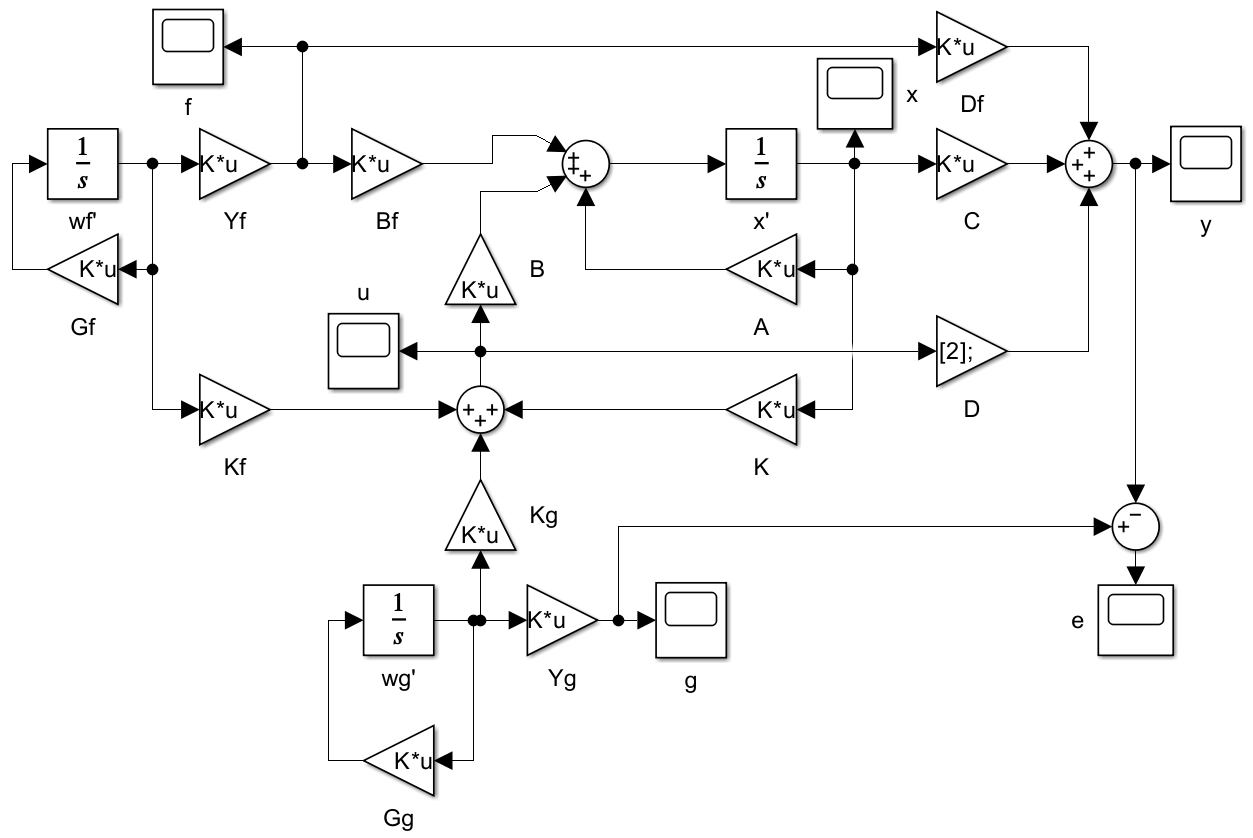
\includegraphics[scale=0.5]{1task_scheme.png}
        \captionsetup{skip=0pt}
        \caption{Схема моделирования системы, замкнутой регулятором}
        \label{fig:1task_scheme}
    \end{figure}
    \noindent Строим графики $f(t),g(t),u(t),x(t),y(t),e(t)$.


    \subsection{Синтез компоненты обратной связи}
    Исследуем систему на стабилизируемость
    $$
    \sigma\left( A \right)=\left\{ -2,2\pm i \right\},\ A_{J_re}=\begin{bmatrix}
        -2 &0 &0\\
        0 &2 &1\\
        0 &-1 &2
    \end{bmatrix},\ B_{J_re}=\begin{bmatrix}
        0\\3\\-1
    \end{bmatrix};
    $$
    Система не полностью управляема, стабилизируема. Максимальная степень
    устойчивости $\alpha=2$.


    Синтезируем компоненту обратной связи $K$ с помощью матричного уравнения
    типа Риккати
    $$
    A^TP+PA+Q-\nu PBR^{-1}B^TP+2\alpha P=0,\,K=-R^{-1}B^TP;
    $$
    при $Q=I,\nu=2,R=1,\alpha=2$. Получаем
    $$
    K=\begin{bmatrix}
        2.1111  &-13.4448    &1.6787
    \end{bmatrix},$$
    $$
    \sigma\left( A+BK \right)=\left\{ -2,-2.3951\pm 4.3138i \right\};
    $$
    Желаемая степень устойчивости достигнута -- регулятор синтезирован корректно.


    \subsection{Общий вид матричных уравнений Франкиса-Дэвисона}
    Матричные уравнения Франкиса-Дэвисона в общем виде представляются системой
    $$
    \begin{cases}
        AP+BK+Y_1=P\Gamma,\\
        CP+DK+Y_2=0;
    \end{cases}
    $$
    Решение относительно $P$ и $K$ для произвольных
    $Y_1$ и $Y_2$ существует, если
    $$
    \text{rank}\left( \mathcal{M} \right)=\text{rank}\begin{bmatrix}
        A-I\lambda_{i\Gamma} &B\\
        C &D
    \end{bmatrix}=\text{число строк}
    $$
    $\lambda_{i\Gamma}$ -- собственные числа $\Gamma$.


    \subsection{Синтез компоненты слежения}
    Проверим условие существования решения
    системы уравнений
    \begin{align}
    \begin{cases}
    P_g\Gamma_g-\left( A+BK \right)P_g=BK_g,\\
    \left( C+DK \right)P_g+DK_g=Y_g;
    \end{cases} \label{eq:Kg}
    \end{align}
    Собственные числа матрицы $\Gamma_g$
    $$
    \sigma\left( \Gamma_g \right)=\left\{ 0,\pm i \right\}
    $$
    Проверим ранги матриц. Выясним количество строк
    $$A_{3\times3},B_{3\times1},K_{1\times3},I_{3\times3},P_{g\,3\times3},C_{1\times3},D_{1\times1}\Rightarrow \mathcal{M}_{4\times4}$$
    Сравниваем ранг с $n=4$
    \begin{align*}
    &\text{rank}\left( \mathcal{M}_{\lambda_1} \right)=\text{rank}\begin{bmatrix}
        \left( A+BK \right)-Ii &B\\
        \left( C+DK \right) &D
    \end{bmatrix}=4,\\
    &\text{rank}\left( \mathcal{M}_{\lambda_2} \right)=\text{rank}\begin{bmatrix}
        \left( A+BK \right)+Ii &B\\
        \left( C+DK \right) &D
    \end{bmatrix}=4,\\
    &\text{rank}\left( \mathcal{M}_{\lambda_3} \right)=\text{rank}\begin{bmatrix}
        \left( A+BK \right)+0I &B\\
        \left( C+DK \right) &D
    \end{bmatrix}=4;
    \end{align*}
    Условие выполнено. Синтезируем компоненту слежения $K_g$ через уравнения (\ref{eq:Kg}).
    Получаем
    $$
    K_g=
    \begin{bmatrix}
        -0.0932   &18.6951   &-8.1152
    \end{bmatrix}
    $$


    \subsection{Синтез компоненты компенсации по входу}
    Проверим условие существования решения системы уравнений
    \begin{align}
        \begin{cases}
            P_f\Gamma_f-\left( A+BK \right)P_f-B_fY_f=BK_f,\\
            \left( C+DK \right)P_f+DK_f=-D_fY_f;
        \end{cases}\label{eq:Kf}
    \end{align}
    Собственные числа матрицы $\Gamma_f$
    $$
    \sigma\left( \Gamma_f \right)=\left\{ \pm i,\pm3i \right\}
    $$
    Сравниваем ранг с $n=4$ (пусть $\left( A+BK \right)=\mathcal{A},\left( C+DK \right)=\mathcal{C}$)
    \begin{align*}
    &\text{rank}\left( \mathcal{M}_{\lambda_1} \right)=\text{rank}\begin{bmatrix}
        \mathcal{A}-Ii &B\\
        \mathcal{C} &D
    \end{bmatrix}=4,\ \text{rank}\left( \mathcal{M}_{\lambda_2} \right)=\text{rank}\begin{bmatrix}
        \mathcal{A}+Ii &B\\
        \mathcal{C} &D
    \end{bmatrix}=4,\\
    &\text{rank}\left( \mathcal{M}_{\lambda_3} \right)=\text{rank}\begin{bmatrix}
        \mathcal{A}-3Ii &B\\
        \mathcal{C} &D
    \end{bmatrix}=4,\ \text{rank}\left( \mathcal{M}_{\lambda_4} \right)=\text{rank}\begin{bmatrix}
        \mathcal{A}+3Ii &B\\
        \mathcal{C} &D
    \end{bmatrix}=4;
    \end{align*}
    Условие выполнено. Синтезируем компоненту компенсации $K_f$ через уравнения (\ref{eq:Kf}).
    Получаем
    $$
    K_f=\begin{bmatrix}
        -725.9021 &-225.1491  &586.1685 &-359.3897
    \end{bmatrix}
    $$


    \subsection{Компьютерное моделирование}
    Промоделируем систему при $u=0,u=Kx,u=Kx+K_fw_f,u=Kx+K_gw_g$ и $u=Kx+K_gw_g+K_fw_f$
    \begin{figure}[H]
        \centering
        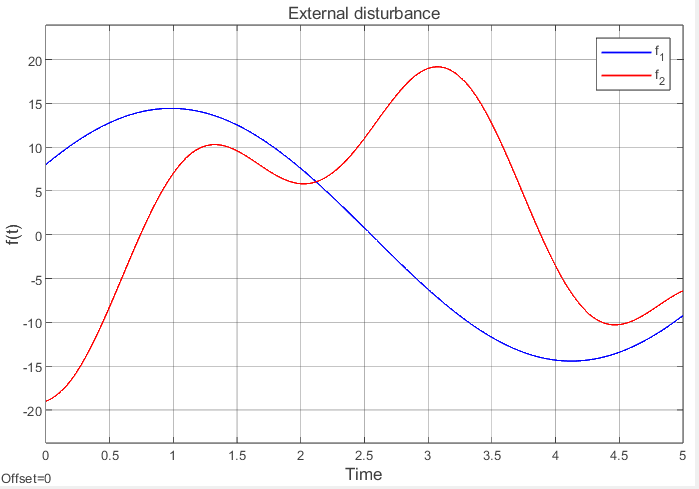
\includegraphics[scale=0.6]{1task_f.png}
        \captionsetup{skip=0pt}
        \caption{График возмущений $f(t)$ для разомкнутой системы $\left( u=0 \right)$}
        \label{fig:1task_f}
    \end{figure}
    \begin{figure}[H]
        \centering
        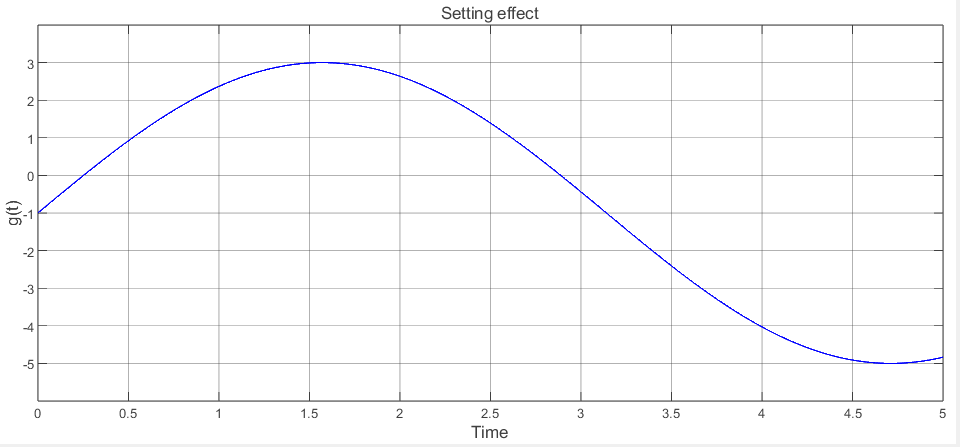
\includegraphics[scale=0.6]{1task_g.png}
        \captionsetup{skip=0pt}
        \caption{График задающего воздействия $g(t)$ для разомкнутой системы $\left( u=0 \right)$}
        \label{fig:1task_g}
    \end{figure}
    \begin{figure}[H]
        \centering
        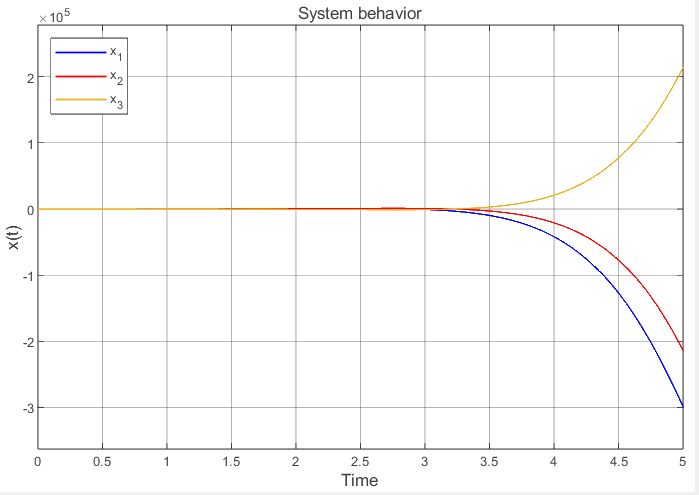
\includegraphics[scale=0.6]{1task_x.png}
        \captionsetup{skip=0pt}
        \caption{График вектора состояния ОУ $x(t)$ для разомкнутой системы $\left( u=0 \right)$}
        \label{fig:1task_x}
    \end{figure}
    \begin{figure}[H]
        \centering
        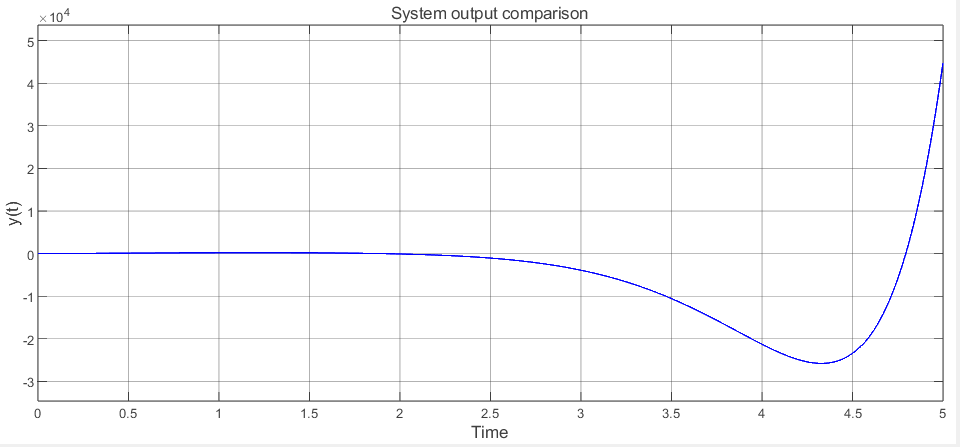
\includegraphics[scale=0.6]{1task_y.png}
        \captionsetup{skip=0pt}
        \caption{График выхода системы $y(t)$ для разомкнутой системы $\left( u=0 \right)$}
        \label{fig:1task_y}
    \end{figure}
    \begin{figure}[H]
        \centering
        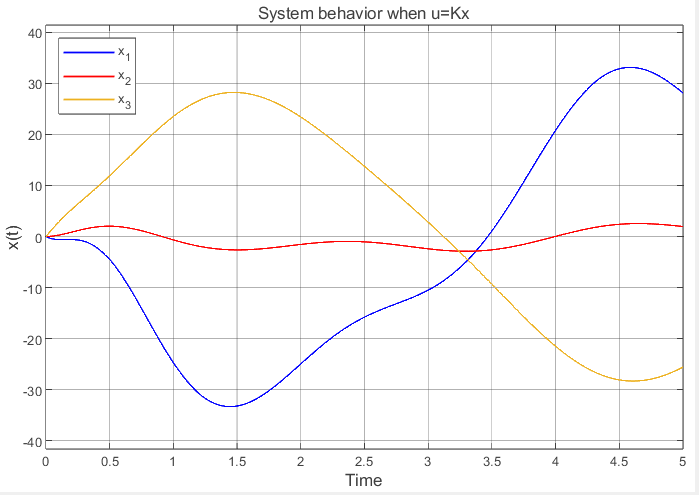
\includegraphics[scale=0.6]{1task_x_kx.png}
        \captionsetup{skip=0pt}
        \caption{График $x(t)$ при $u=Kx$}
        \label{fig:1task_x_kx}
    \end{figure}
    \begin{figure}[H]
        \centering
        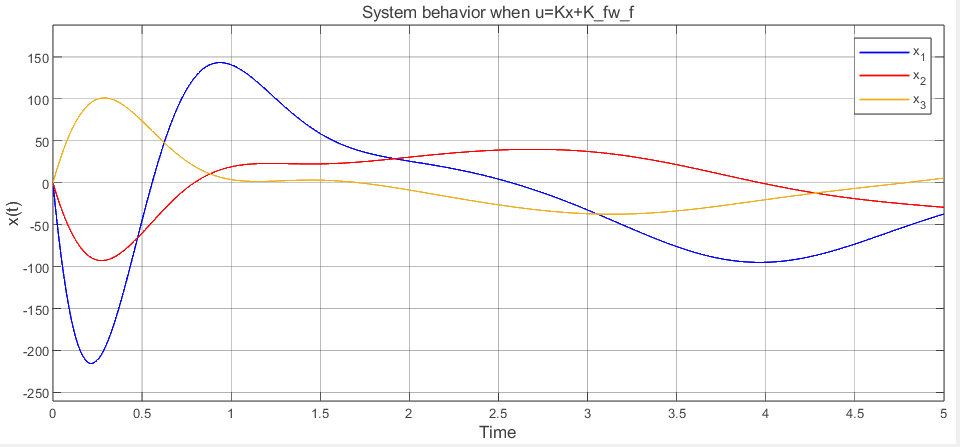
\includegraphics[scale=0.6]{1task_x_kxkf.png}
        \captionsetup{skip=0pt}
        \caption{График $x(t)$ при $u=Kx+K_fw_f$}
        \label{fig:1task_x_kxkf}
    \end{figure}
    \begin{figure}[H]
        \centering
        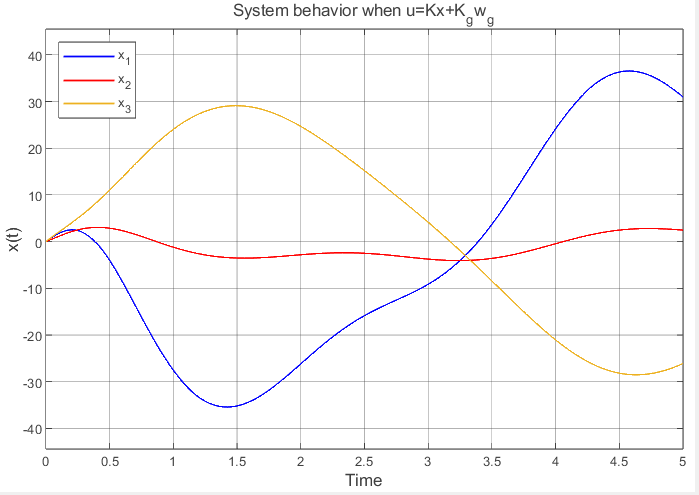
\includegraphics[scale=0.6]{1task_x_kxkg.png}
        \captionsetup{skip=0pt}
        \caption{График $x(t)$ при $u=Kx+K_gw_g$}
        \label{fig:1task_x_kxkg}
    \end{figure}
    \begin{figure}[H]
        \centering
        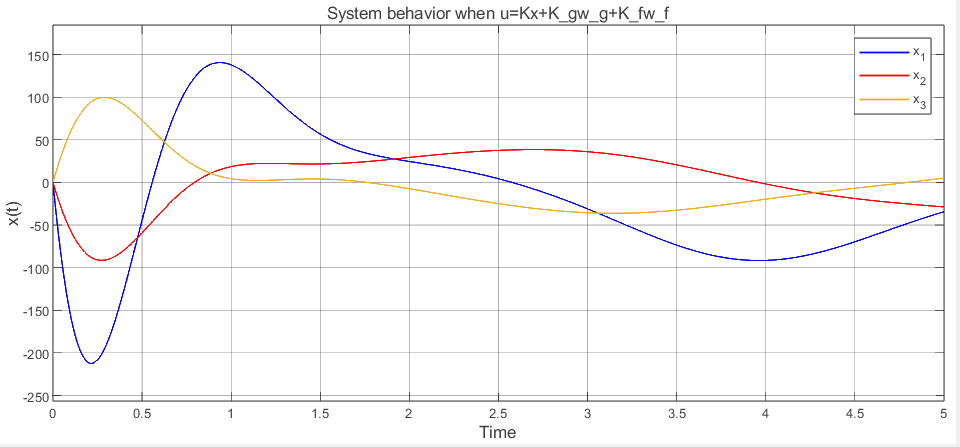
\includegraphics[scale=0.6]{1task_x_kxkgkf.png}
        \captionsetup{skip=0pt}
        \caption{График $x(t)$ при $u=Kx+K_gw_g+K_fw_f$}
        \label{fig:1task_x_kxkgkf}
    \end{figure}
    \begin{figure}[H]
        \centering
        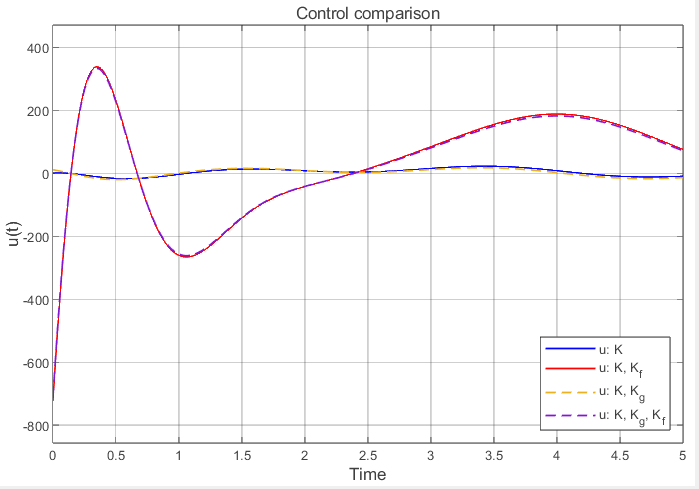
\includegraphics[scale=0.6]{1task_u.png}
        \captionsetup{skip=0pt}
        \caption{Сравнение графиков $u(t)$ для замкнутых систем}
        \label{fig:1task_u}
    \end{figure}
    \begin{figure}[H]
        \centering
        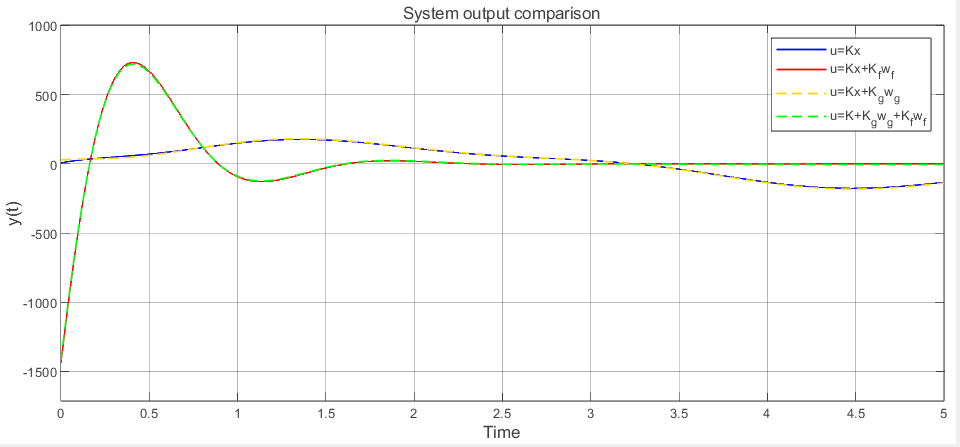
\includegraphics[scale=0.6]{1task_yy.png}
        \captionsetup{skip=0pt}
        \caption{Сравнение графиков $y(t)$ для замкнутых систем}
        \label{fig:1task_yy}
    \end{figure}
    \begin{figure}[H]
        \centering
        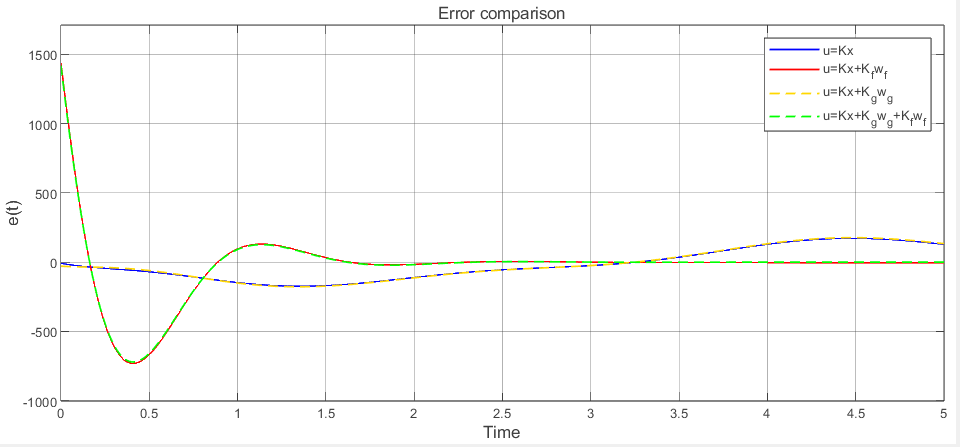
\includegraphics[scale=0.6]{1task_e.png}
        \captionsetup{skip=0pt}
        \caption{Сравнение графиков $e(t)=g(t)-y(t)$ для замкнутых систем}
        \label{fig:1task_e}
    \end{figure}


    \subsection{Сравнение результатов}
    При отсутствии управления объект управления разошелся.
    При наличии в управлении всех компонент выход системы $y(t)$
    удалось свести к задающему воздействию $g(t)$. Результат
    при $K,K_f$ схож с результатом при всех компонентах.
    Также схожи результаты при $K$ и $K,K_g$.


    \section{Задание 2. Слежение и компенсация по выходу}
    Рассмотрим систему (\ref{eq:sys1}),
    генератор внешнего возмущения (\ref{eq:sys12}) и
    генератор задающего воздействия (\ref{eq:sys13}).
    Матрицы $K,K_g,K_f$ используем как в первом задании
    \begin{align*}
    &K=\begin{bmatrix}
        2.1111  &-13.4448    &1.6787
    \end{bmatrix},\\
    &K_g=
    \begin{bmatrix}
        -0.0932   &18.6951   &-8.1152
    \end{bmatrix},\\
    &K_f=\begin{bmatrix}
        -725.9021 &-225.1491  &586.1685 &-359.3897
    \end{bmatrix};
    \end{align*}
    Программа для задания 2 представлена в приложении Б на листинге \ref{task2}.


    \subsection{Схема моделирования системы}
    Система замкнута регулятором,
    состоящим из наблюдателя задающего воздействия,
    наблюдателя расширенной размерности
    и закона управления
    $$
    u=K\hat{x}+K_g\hat{w}_g+K_f\hat{w}_f,
    $$
    обеспечивающим выполнение целевого условия (\ref{eq:aim}).
    Строим график формируемого регулятором
    управления $u(t)$, сравнительные графики
    $$
    \begin{bmatrix}
        w_f(t)\\x(t)
    \end{bmatrix}\text{ и }\begin{bmatrix}
        \hat{w}_f(t)\\ \hat{x}(t)
    \end{bmatrix},
    $$
    график ошибки наблюдателя расширенной размерности
    $$
    e_f(t)=\begin{bmatrix}
        w_f(t)\\x(t)
    \end{bmatrix}-\begin{bmatrix}
        \hat{w}_f(t)\\ \hat{x}(t)
    \end{bmatrix},
    $$
    сравнительные графики $w_g(t)$ и $\hat{w}_g(t)$, график
    ошибки наблюдателя задающего воздействия $$e_g(t)=w_g(t)-\hat{w}_g(t),$$
    график выхода $y(t)$ и график ошибки управления $$e(t)=g(t)-y(t)$$
    Схема представлена на рис. \ref{fig:2task_scheme}
    \begin{figure}[H]
        \centering
        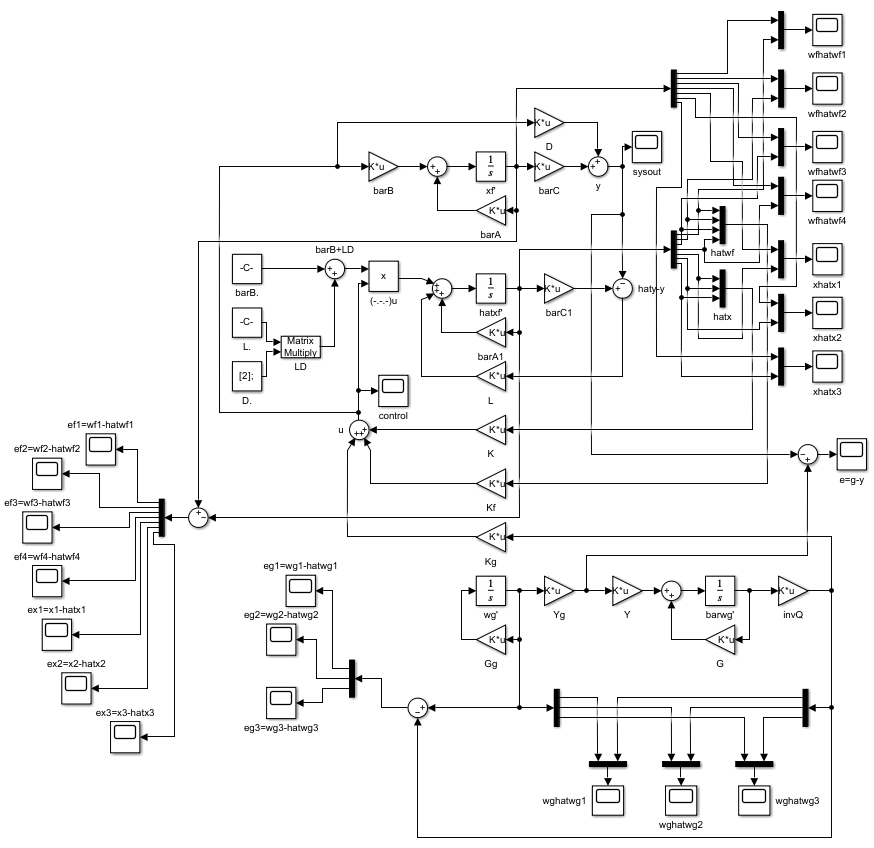
\includegraphics[scale=0.75]{2task_scheme.png}
        \captionsetup{skip=0pt}
        \caption{Схема моделирования системы, замкнутой регулятором}
        \label{fig:2task_scheme}
    \end{figure}


    \subsection{Наблюдатель задающего воздействия}
    Зададим желаемую динамику наблюдателя $\left( \Gamma,Y \right)$, где $\Gamma$ -- гурвицева
    $$
    \Gamma=\begin{bmatrix}
        -1 &0 &0\\
        0 &-5 &0\\
        0 &0 &-10
    \end{bmatrix},\ Y=\begin{bmatrix}
        1\\1\\1
    \end{bmatrix};
    $$
    $\Gamma$ определяет скорость схождения ошибки $\tilde{w}_g=w_g-\hat{w}_g$ к 0. Цель
    $$
    \lim\limits_{t\to\infty}||w_g(t)-\hat{w}_g(t)||=0
    $$
    Наблюдатель сигнала задания
    $$
    \dot{\bar{w}}_g=\Gamma\bar{w}_g+Yg
    $$
    Найдем матрицу смены базиса $Q$
    $$
    \bar{w}_g=Q\hat{w}_g
    $$
    через уравнение типа Сильвестра
    $$
    Q\Gamma_g-\Gamma Q=YY_g
    $$
    Получаем
    $$
    Q=\begin{bmatrix}
        2.0000   &-2.0000   &-1.0000\\
    0.7692   &-0.1538   &-0.2000\\
    0.3960   &-0.0396   &-0.1000
    \end{bmatrix},\ Q^{-1}=\begin{bmatrix}
        -0.6806   &14.6250  &-22.4444\\
    0.2083  &-17.8750   &33.6667\\
   -2.7778   &65.0000 &-112.2222
    \end{bmatrix};
    $$


    \subsection{Синтез наблюдателя расширенной размерности}
    Сформируем расширенную систему
    $$
    x_f=\begin{bmatrix}
        w_f\\
        x
    \end{bmatrix},\ \bar{A}=\begin{bmatrix}
        \Gamma_f &0_{4\times3}\\
        B_fY_f &A
    \end{bmatrix},\ \bar{B}=\begin{bmatrix}
        0_{4\times1}\\B
    \end{bmatrix},\ \bar{C}=\begin{bmatrix}
        D_fY_f &C
    \end{bmatrix};
    $$
    Наблюдатель повышенной размерности
    $$
    \begin{cases}
        \dot{\hat{x}}_f=\bar{A}\hat{x}_f+\left( \bar{B}+LD \right)u+L\left( \hat{y}-y \right),\\
        \hat{y}=\bar{C}\hat{x}_f;
    \end{cases}
    $$
    Синтезируем матрицу коррекции наблюдателя путем решения матричного уравнения
    типа Риккати
    $$
    \bar{A}P+P\bar{A}^T+Q_{L}-\nu P\bar{C}^TR^{-1}\bar{C}P=0,\ L=-P\bar{C}^TR^{-1}
    $$
    При $Q_{L}=I_{7\times7},\ R=1,\ \nu=1$ получаем
    $$
    L=10^3\cdot\begin{bmatrix}
    -0.0066&
    0.0219&
   -0.0143&
   -0.0229&
    1.7022&
    1.0491&
   -1.0838
    \end{bmatrix}^T
    $$

    
    % pos 389.8,229.8,768,357.6
    \subsection{Компьютерное моделирование}
    Зададим нулевые начальные условия наблюдателей и выполним компьютерное моделирование замкнутой системы
    \begin{figure}[H]
        \centering
        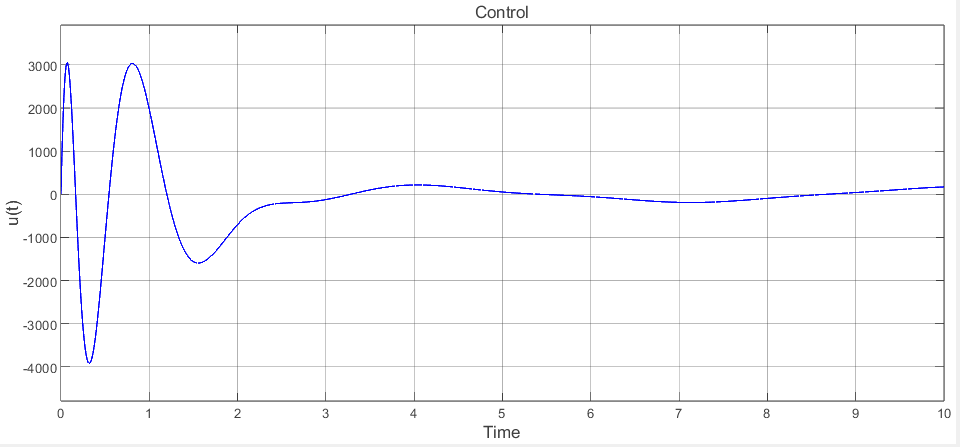
\includegraphics[scale=0.6]{2task_u.png}
        \captionsetup{skip=0pt}
        \caption{График управления $u(t)$}
        \label{fig:2task_u}
    \end{figure}
    \begin{figure}[H]
        \centering
        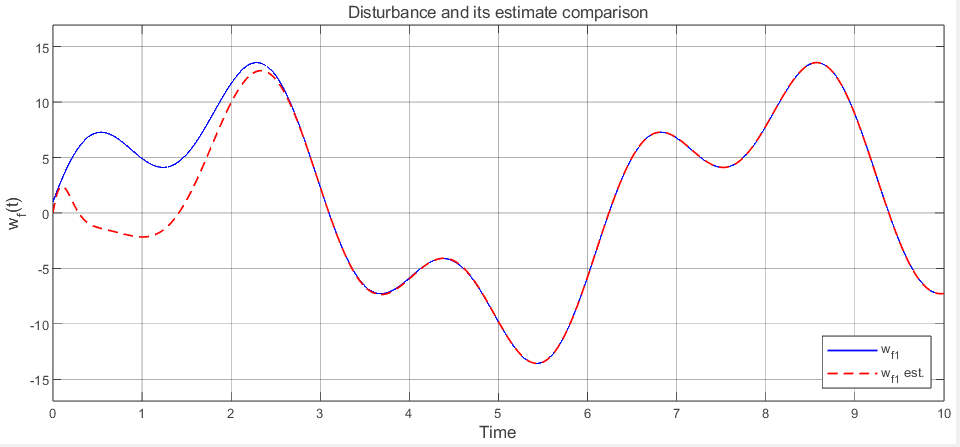
\includegraphics[scale=0.6]{2task_wfhwf1.png}
        \captionsetup{skip=0pt}
        \caption{График возмущения $w_{f_1}(t)$ и его оценки $\hat{w}_{f_1}(t)$}
        \label{fig:2task_wfhwf1}
    \end{figure}
    \begin{figure}[H]
        \centering
        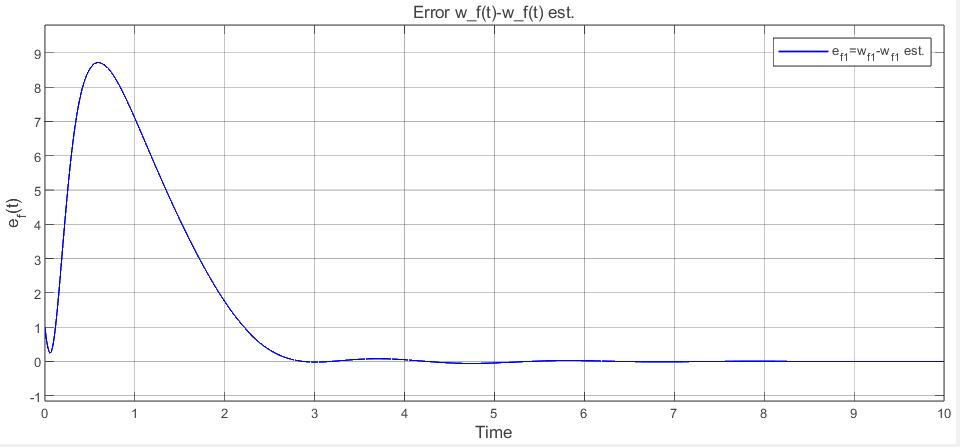
\includegraphics[scale=0.6]{2task_ef1.png}
        \captionsetup{skip=0pt}
        \caption{График ошибки $e_{f_1}(t)=w_{f_1}(t)-\hat{w}_{f_1}(t)$}
        \label{fig:2task_ef1}
    \end{figure}
    \begin{figure}[H]
        \centering
        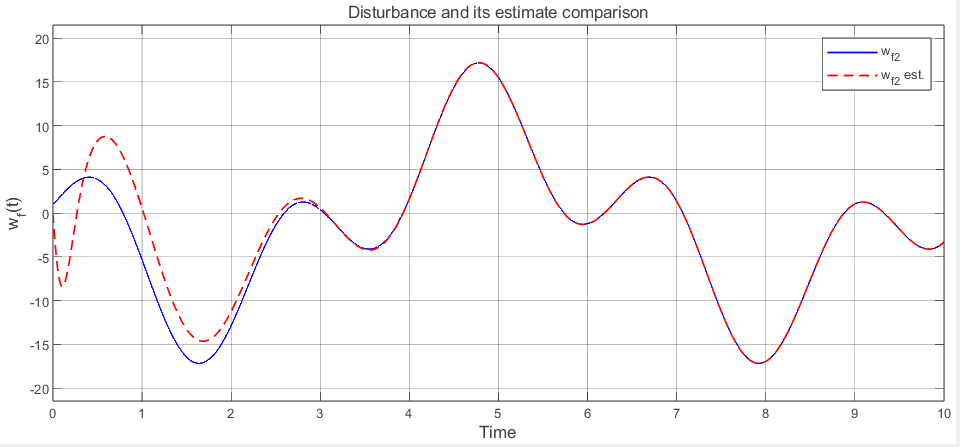
\includegraphics[scale=0.6]{2task_wfhwf2.png}
        \captionsetup{skip=0pt}
        \caption{График возмущения $w_{f_2}(t)$ и его оценки $\hat{w}_{f_2}(t)$}
        \label{fig:2task_wfhwf2}
    \end{figure}
    \begin{figure}[H]
        \centering
        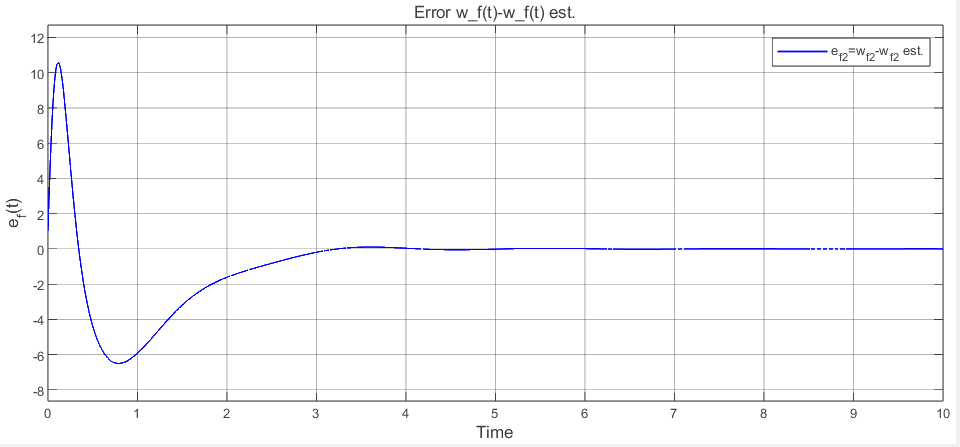
\includegraphics[scale=0.6]{2task_ef2.png}
        \captionsetup{skip=0pt}
        \caption{График ошибки $e_{f_2}(t)=w_{f_2}(t)-\hat{w}_{f_2}(t)$}
        \label{fig:2task_ef2}
    \end{figure}
    \begin{figure}[H]
        \centering
        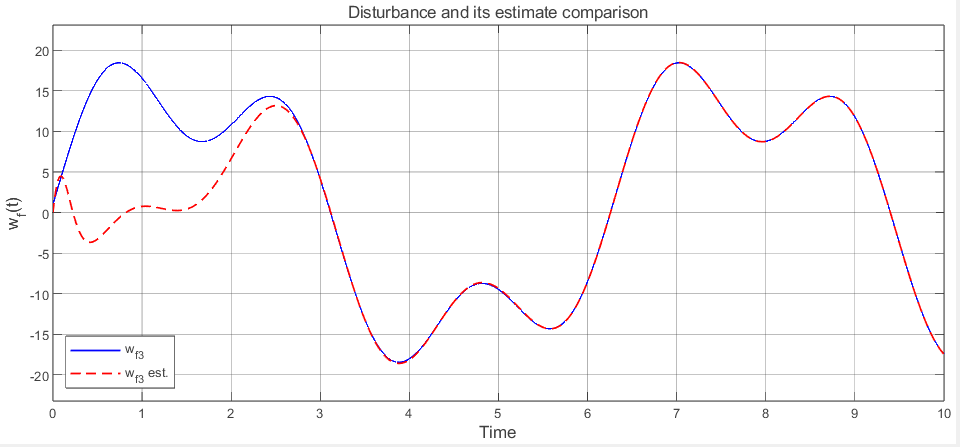
\includegraphics[scale=0.6]{2task_wfhwf3.png}
        \captionsetup{skip=0pt}
        \caption{График возмущения $w_{f_3}(t)$ и его оценки $\hat{w}_{f_3}(t)$}
        \label{fig:2task_wfhwf3}
    \end{figure}
    \begin{figure}[H]
        \centering
        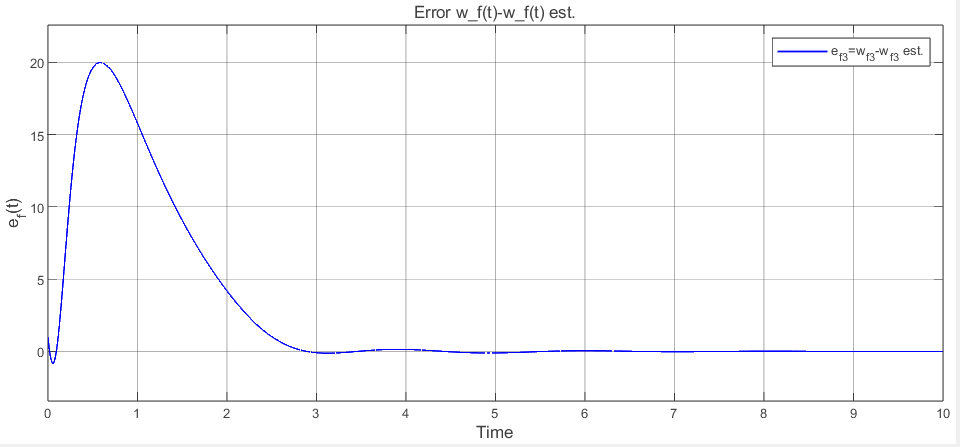
\includegraphics[scale=0.6]{2task_ef3.png}
        \captionsetup{skip=0pt}
        \caption{График ошибки $e_{f_3}(t)=w_{f_3}(t)-\hat{w}_{f_3}(t)$}
        \label{fig:2task_ef3}
    \end{figure}
    \begin{figure}[H]
        \centering
        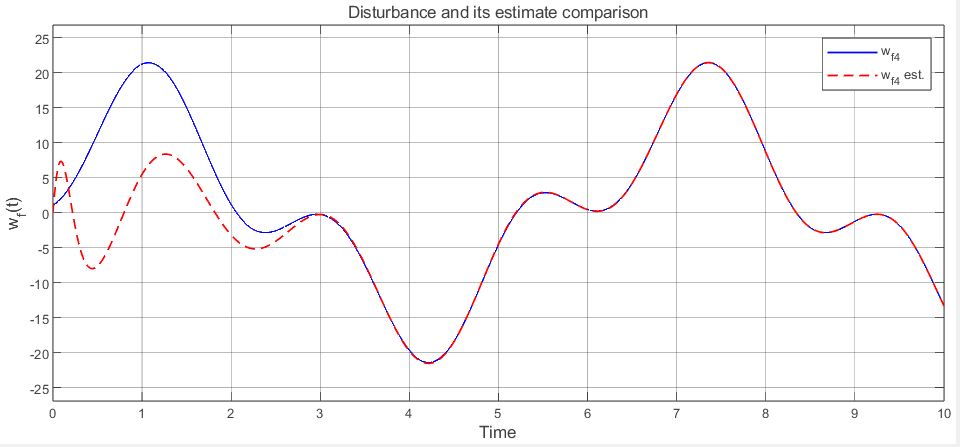
\includegraphics[scale=0.6]{2task_wfhwf4.png}
        \captionsetup{skip=0pt}
        \caption{График возмущения $w_{f_4}(t)$ и его оценки $\hat{w}_{f_4}(t)$}
        \label{fig:2task_wfhwf4}
    \end{figure}
    \begin{figure}[H]
        \centering
        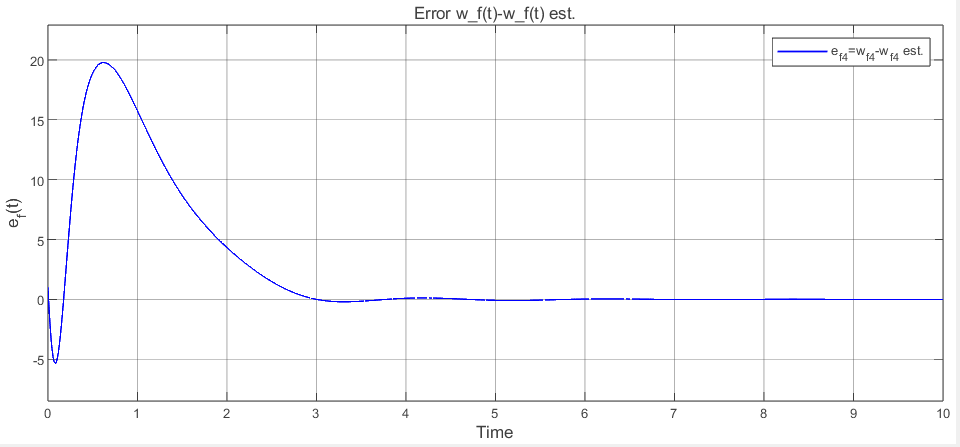
\includegraphics[scale=0.6]{2task_ef4.png}
        \captionsetup{skip=0pt}
        \caption{График ошибки $e_{f_4}(t)=w_{f_4}(t)-\hat{w}_{f_4}(t)$}
        \label{fig:2task_ef4}
    \end{figure}
    \begin{figure}[H]
        \centering
        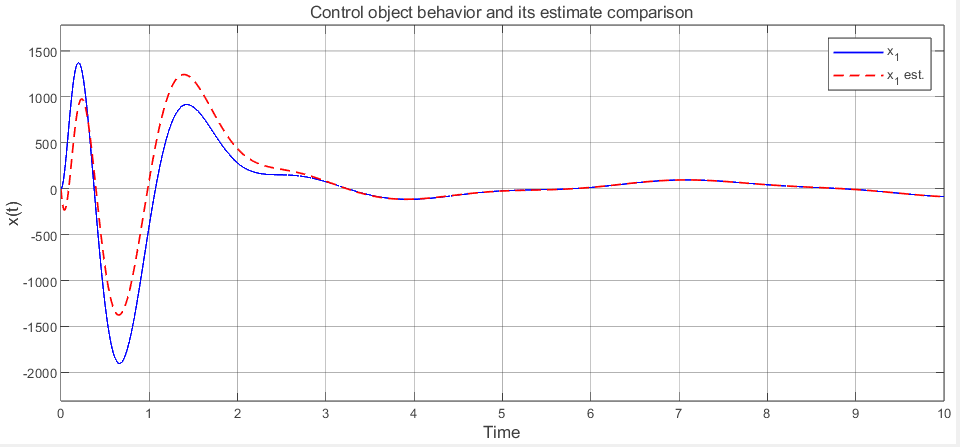
\includegraphics[scale=0.6]{2task_xhx1.png}
        \captionsetup{skip=0pt}
        \caption{График координаты вектора состояния ОУ $x_{1}(t)$ и ее оценки $\hat{x}_{1}(t)$}
        \label{fig:2task_xhx1}
    \end{figure}
    \begin{figure}[H]
        \centering
        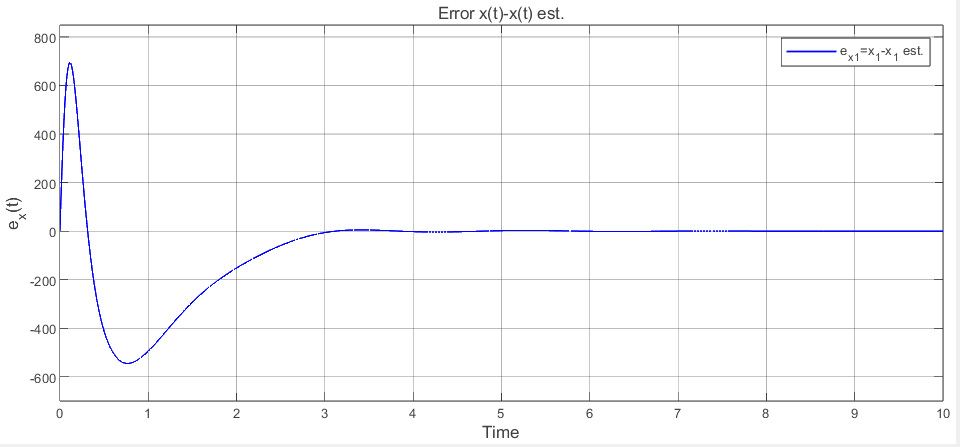
\includegraphics[scale=0.6]{2task_ex1.png}
        \captionsetup{skip=0pt}
        \caption{График ошибки $e_{x_1}(t)=x_{1}(t)-\hat{x}_{1}(t)$}
        \label{fig:2task_ex1}
    \end{figure}
    \begin{figure}[H]
        \centering
        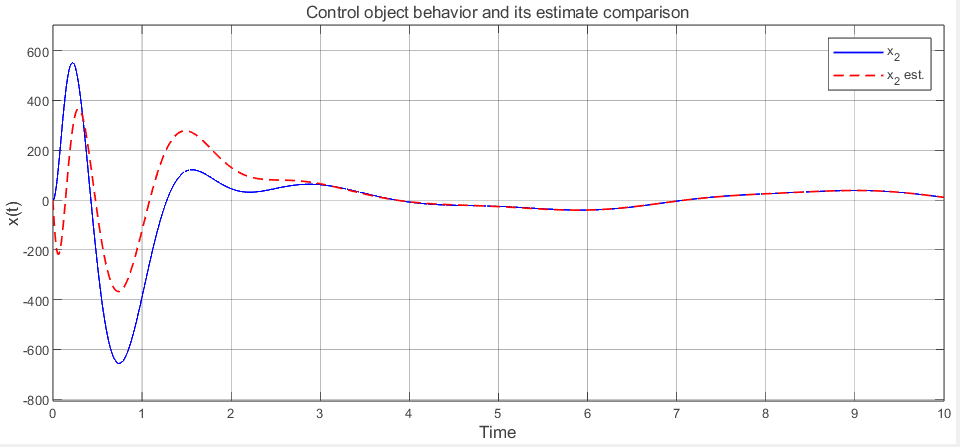
\includegraphics[scale=0.6]{2task_xhx2.png}
        \captionsetup{skip=0pt}
        \caption{График координаты вектора состояния ОУ $x_{2}(t)$ и ее оценки $\hat{x}_{2}(t)$}
        \label{fig:2task_xhx2}
    \end{figure}
    \begin{figure}[H]
        \centering
        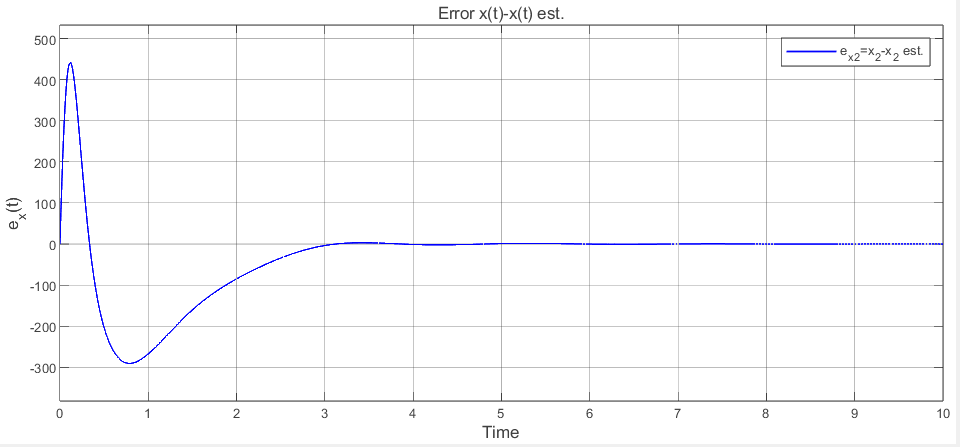
\includegraphics[scale=0.6]{2task_ex2.png}
        \captionsetup{skip=0pt}
        \caption{График ошибки $e_{x_2}(t)=x_{2}(t)-\hat{x}_{2}(t)$}
        \label{fig:2task_ex2}
    \end{figure}
    \begin{figure}[H]
        \centering
        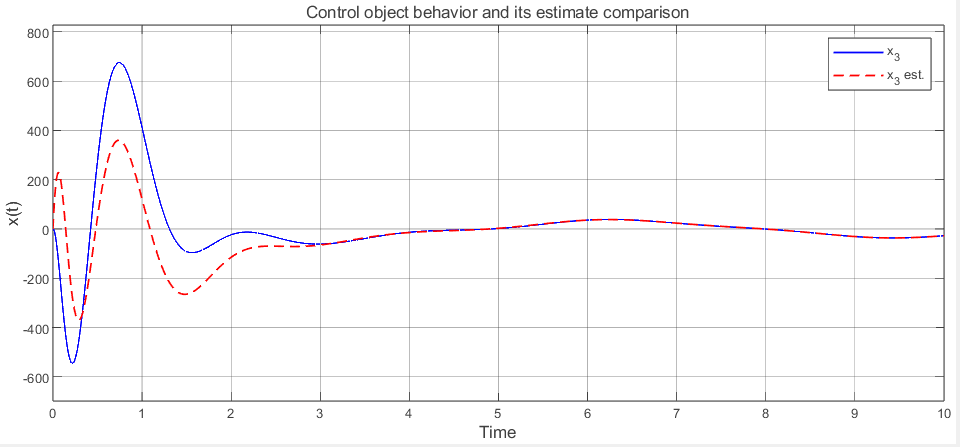
\includegraphics[scale=0.6]{2task_xhx3.png}
        \captionsetup{skip=0pt}
        \caption{График координаты вектора состояния ОУ $x_{3}(t)$ и ее оценки $\hat{x}_{3}(t)$}
        \label{fig:2task_xhx3}
    \end{figure}
    \begin{figure}[H]
        \centering
        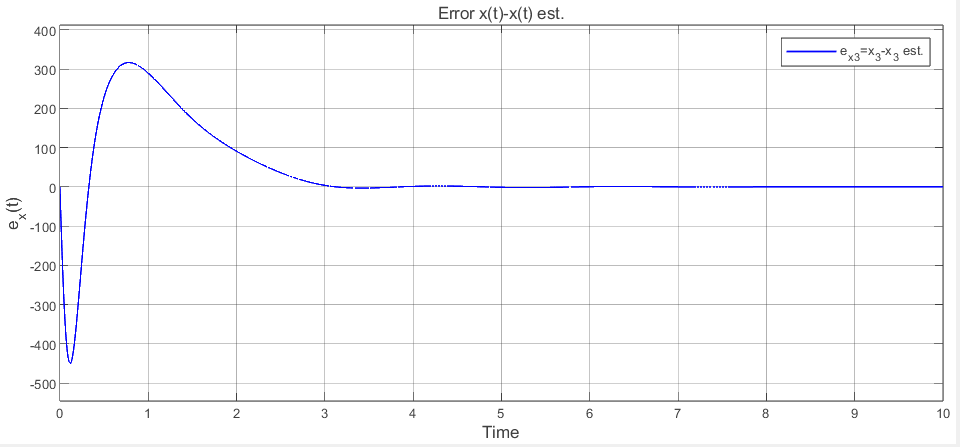
\includegraphics[scale=0.6]{2task_ex3.png}
        \captionsetup{skip=0pt}
        \caption{График ошибки $e_{x_3}(t)=x_{3}(t)-\hat{x}_{3}(t)$}
        \label{fig:2task_ex3}
    \end{figure}
    \begin{figure}[H]
        \centering
        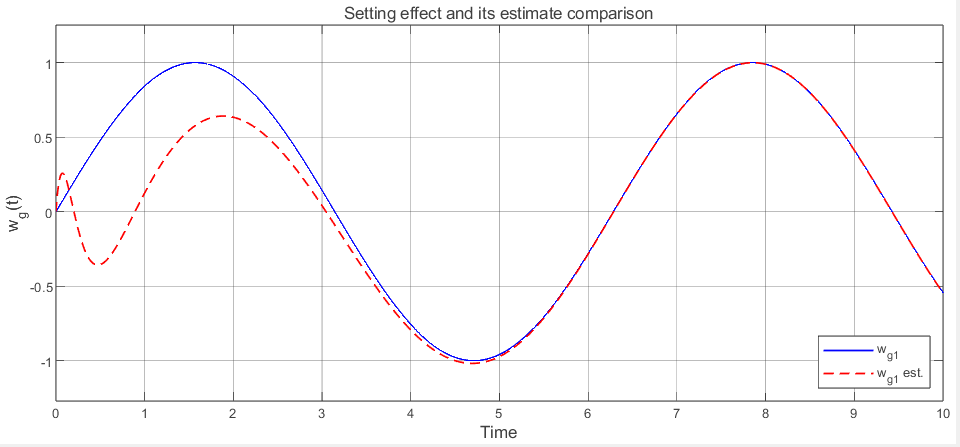
\includegraphics[scale=0.6]{2task_wghwg1.png}
        \captionsetup{skip=0pt}
        \caption{График задающего воздействия $w_{g_1}(t)$ и его оценки $\hat{w}_{g_1}(t)$}
        \label{fig:2task_wghwg1}
    \end{figure}
    \begin{figure}[H]
        \centering
        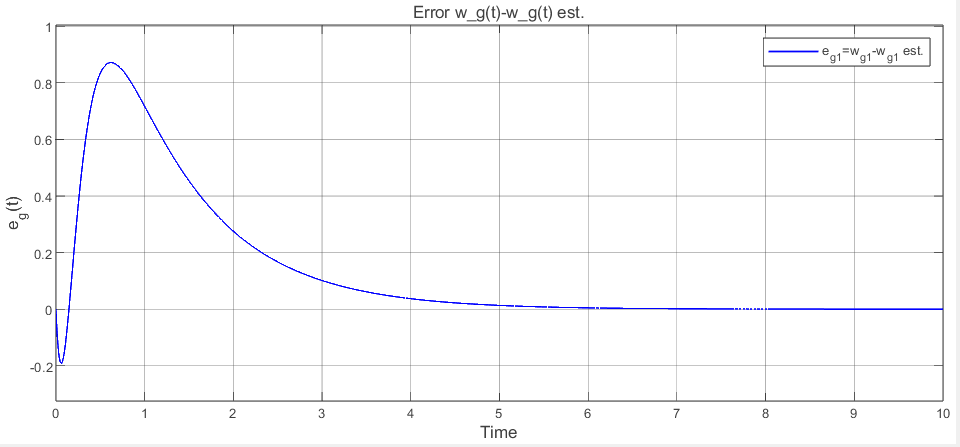
\includegraphics[scale=0.6]{2task_eg1.png}
        \captionsetup{skip=0pt}
        \caption{График ошибки $e_{g_1}(t)=w_{g_1}(t)-\hat{w}_{g_1}(t)$}
        \label{fig:2task_eg1}
    \end{figure}
    \begin{figure}[H]
        \centering
        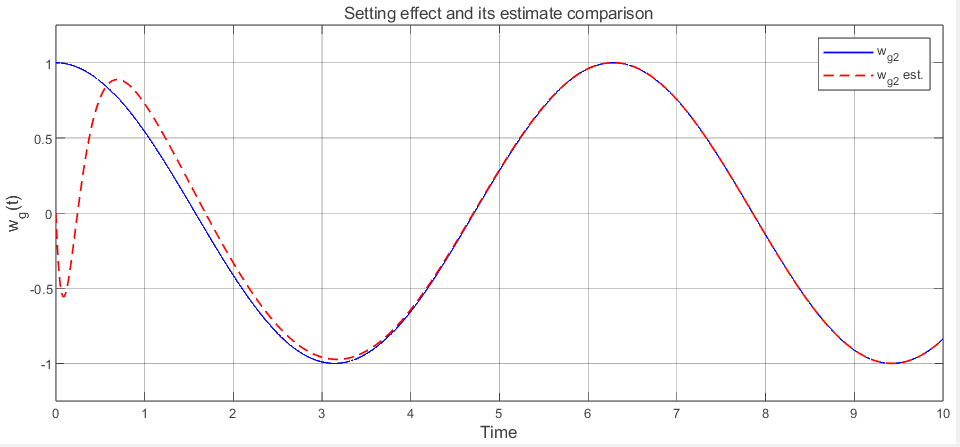
\includegraphics[scale=0.6]{2task_wghwg2.png}
        \captionsetup{skip=0pt}
        \caption{График задающего воздействия $w_{g_2}(t)$ и его оценки $\hat{w}_{g_2}(t)$}
        \label{fig:2task_wghwg2}
    \end{figure}
    \begin{figure}[H]
        \centering
        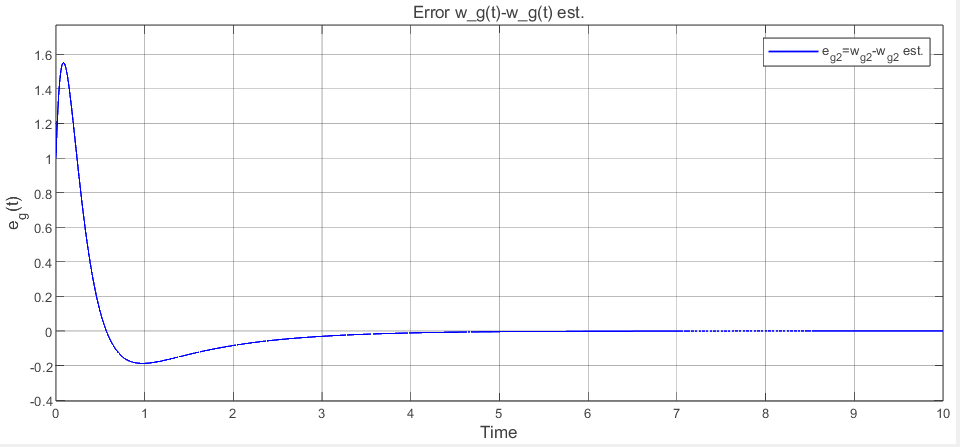
\includegraphics[scale=0.6]{2task_eg2.png}
        \captionsetup{skip=0pt}
        \caption{График ошибки $e_{g_2}(t)=w_{g_2}(t)-\hat{w}_{g_2}(t)$}
        \label{fig:2task_eg2}
    \end{figure}
    \begin{figure}[H]
        \centering
        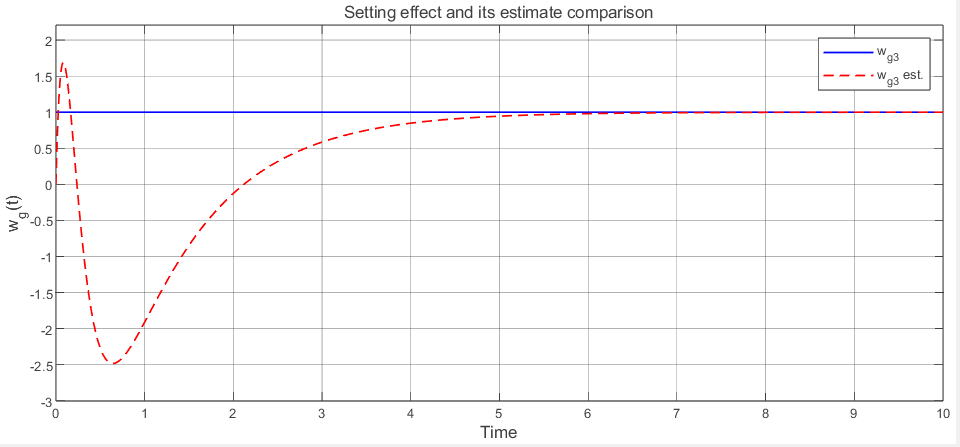
\includegraphics[scale=0.6]{2task_wghwg3.png}
        \captionsetup{skip=0pt}
        \caption{График задающего воздействия $w_{g_3}(t)$ и его оценки $\hat{w}_{g_3}(t)$}
        \label{fig:2task_wghwg3}
    \end{figure}
    \begin{figure}[H]
        \centering
        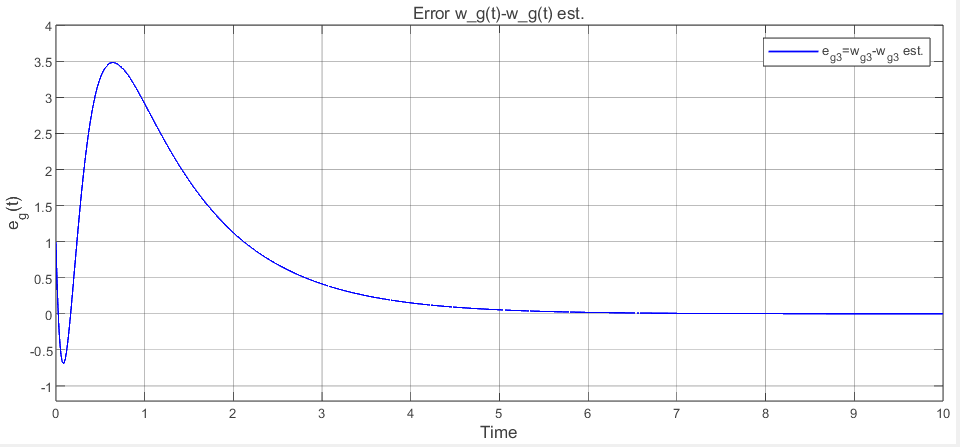
\includegraphics[scale=0.6]{2task_eg3.png}
        \captionsetup{skip=0pt}
        \caption{График ошибки $e_{g_3}(t)=w_{g_3}(t)-\hat{w}_{g_3}(t)$}
        \label{fig:2task_eg3}
    \end{figure}
    \begin{figure}[H]
        \centering
        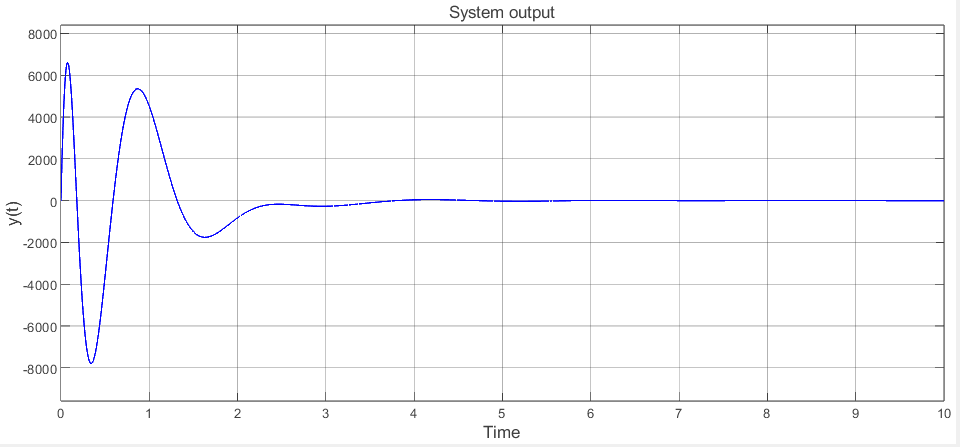
\includegraphics[scale=0.6]{2task_y.png}
        \captionsetup{skip=0pt}
        \caption{График выхода $y(t)$}
        \label{fig:2task_y}
    \end{figure}
    \begin{figure}[H]
        \centering
        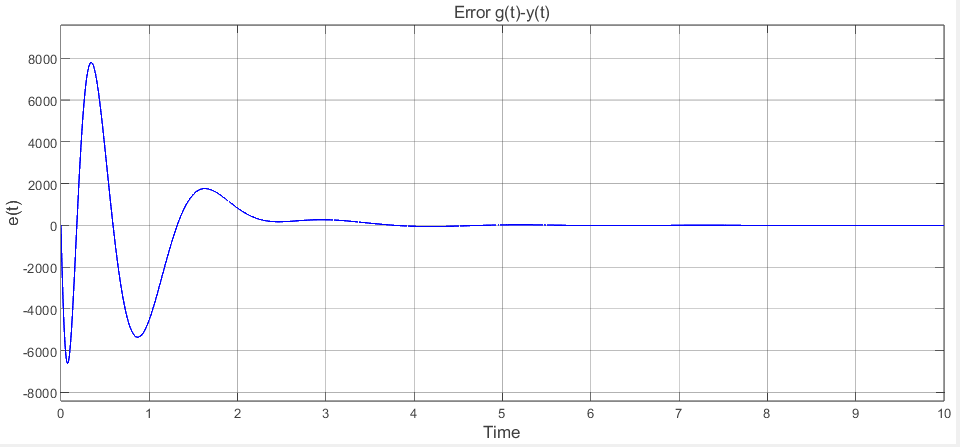
\includegraphics[scale=0.6]{2task_ey.png}
        \captionsetup{skip=0pt}
        \caption{График ошибки $e(t)=g(t)-y(t)$}
        \label{fig:2task_ey}
    \end{figure}


    \subsection{Сравнение результатов}
    Все оценки наблюдателей сошлись к соответствующим истинным траекториям.
    Все ошибки со временим свелись к нулю. В сравнении с заданием 1 выход системы
    имеет больше осцилляций, управления затрачивается сравнительно больше.
    Тем не менее такая модель лучше, так как мы не используем истинные метки,
    а оцениваем их по некоторой доступной информации.


    \section{Задание 3. Слежение и компенсация: наблюдатели возмущения}
    Рассмотрим систему (\ref{eq:sys1}), генератор внешнего возмущения
    (\ref{eq:sys12}) и генератор задающего воздействия (\ref{eq:sys13}).
    Матрицы $K,K_g,K_f,Q$ используем из предыдущих заданий
    \begin{align*}
        &K=\begin{bmatrix}
            2.1111  &-13.4448    &1.6787
        \end{bmatrix},\\
        &K_g=
        \begin{bmatrix}
            -0.0932   &18.6951   &-8.1152
        \end{bmatrix},\\
        &K_f=\begin{bmatrix}
            -725.9021 &-225.1491  &586.1685 &-359.3897
        \end{bmatrix},\\
        &Q=\begin{bmatrix}
            2.0000   &-2.0000   &-1.0000\\
    0.7692   &-0.1538   &-0.2000\\
    0.3960   &-0.0396   &-0.1000
        \end{bmatrix};
    \end{align*}
    Считаем вектор состояния системы $x(t)$ доступным к измерению.
    Программа расположена в приложении В на листинге \ref{task3}.


    \subsection{Наблюдатель возмущения по состоянию}
    Наблюдатель редуцированной размерности
    \begin{align}
    \begin{cases}
        \hat{w}_f=\hat{z}+L\bar{C}x,\\
        \dot{\hat{z}}=F\hat{z}+\left( FL\bar{C}-L\bar{C}A \right)x-L\bar{C}Bu,
    \end{cases} \bar{C}B_f=I;\label{eq:sys}
    \end{align}
    Нужны соотношения
    \begin{align}
    &F=\Gamma_f-LY_f\text{ (чтобы сгруппировать)},\label{eq:F1} \\
    &Q_LFQ_L^{-1}=\Gamma\text{ (для желаемой динамики)}; \label{eq:F2}
    \end{align}
    Для синтеза $Q_L,L$ понадобится уравнение типа Сильвестра
    \begin{align}
    Q_L\Gamma-\Gamma_f^TQ_L=Y_f^TY,\ L^T=-YQ_L^{-1};\label{eq:sylv}
    \end{align}
    Зададимся желаемой динамикой $\left( \Gamma_{4\times4},Y_{2\times4} \right)$
    $$
    \Gamma=\begin{bmatrix}
        -0.5 &0 &0 &0\\
        0 &-1 &0 &0\\
        0 &0 &-1.5 &0\\
        0 &0 &0 &-2
    \end{bmatrix},\ Y=\begin{bmatrix}
        1 &0 &1 &0\\
        0 &1 &0 &1
    \end{bmatrix};
    $$
    Решим уравнение Сильвестра (\ref{eq:sylv}) относительно $Q_L$ и найдем $L$
    $$
    Q_L=\begin{bmatrix}
    6.4000   &10.2000   &-0.0000    &7.1692\\
    2.4000    &3.2000    &0.3077    &2.3077\\
   -5.6000   &-8.0000   &-0.3077   &-5.6615\\
    3.2000    &5.0000   &-0.0000    &3.4308
    \end{bmatrix},\ L=\begin{bmatrix}
    1.2833   &-2.6667\\
   -5.6583   &-2.3333\\
   -2.4083   &-2.3333\\
   -2.8500    &3.0000
    \end{bmatrix};
    $$
    Определим $\bar{C}$ и $F$ из формул (\ref{eq:sys}), (\ref{eq:F1})
    $$
    \bar{C}=\begin{bmatrix}
    0 &0 &0.25\\
   -1 &0 &-1
    \end{bmatrix},\ F=\begin{bmatrix}
    -38.6000  &-12.5667   &30.3667  &-18.1333\\
   12.6000    &0.3167   &-6.6167    &5.6333\\
   12.6000    &1.8167   &-8.1167    &5.6333\\
   88.8000   &27.7000  &-69.1000   &41.4000
    \end{bmatrix};
    $$


    \subsection{Схема моделирования системы с наблюдателем возмущения по состоянию. Компьютерное моделирование системы}
    Система замкнута регулятором, состоящим из наблюдателя задающего воздействия, 
    наблюдателя возмущения по состоянию и закона управления $u=Kx+K_g\hat{w}_g+K_f\hat{w}_f,$
    обеспечивающим выполнение целевого условия (\ref{eq:aim}). Снимем графики $u(t)$, $x(t)$, $w_f(t)$, $\hat{w}_f(t)$, $e_f(t)$, $e(t)$
    \begin{figure}[H]
        \centering
        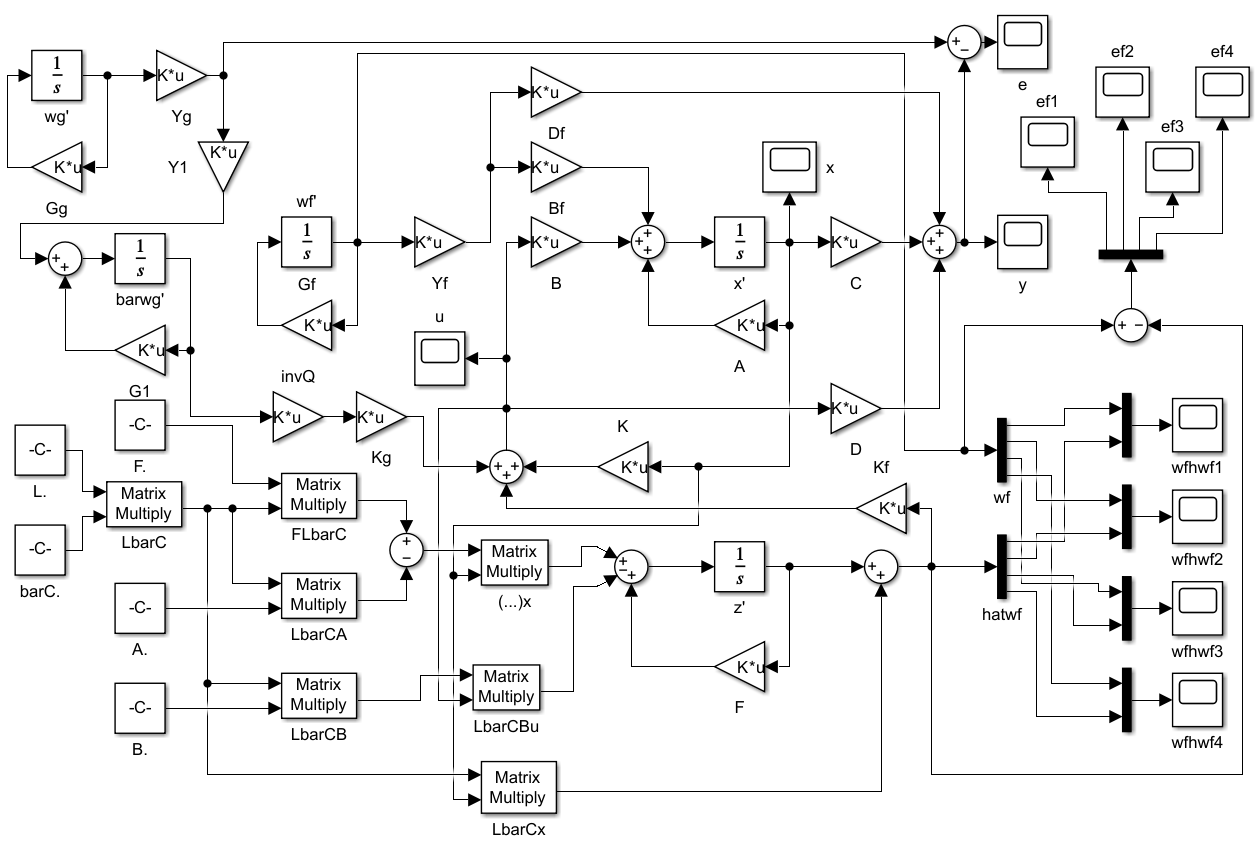
\includegraphics[scale=0.5]{3task_scheme_1.png}
        \captionsetup{skip=0pt}
        \caption{Схема моделирования системы с наблюдателем возмущения по состоянию}
        \label{fig:3task_scheme_1}
    \end{figure}
    \begin{figure}[H]
        \centering
        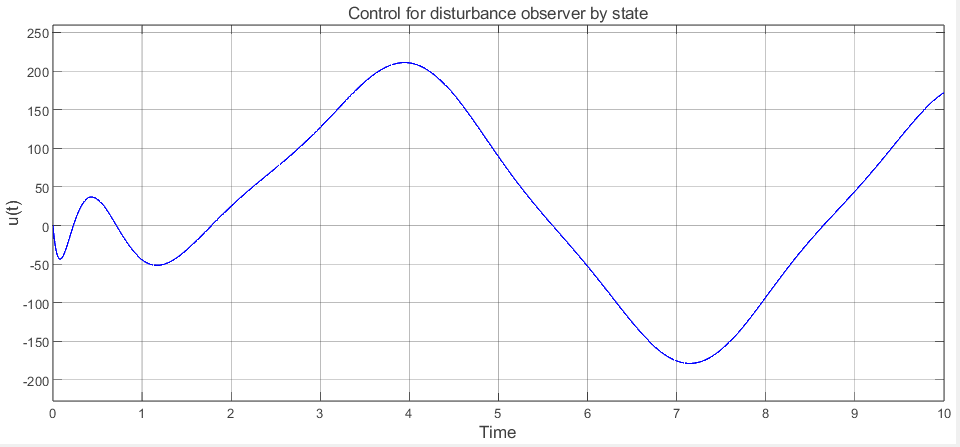
\includegraphics[scale=0.6]{3task_u1.png}
        \captionsetup{skip=0pt}
        \caption{График управления $u(t)$ (набл. возм. по сост.)}
        \label{fig:3task_u1}
    \end{figure}
    \begin{figure}[H]
        \centering
        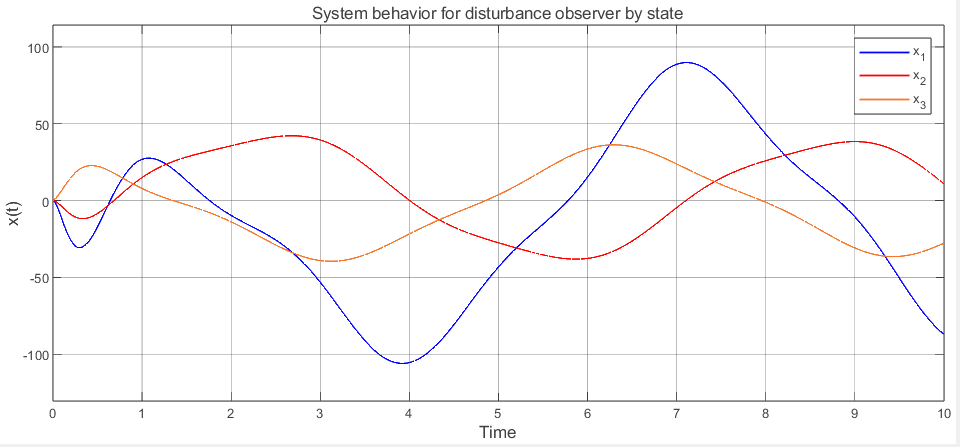
\includegraphics[scale=0.6]{3task_x1.png}
        \captionsetup{skip=0pt}
        \caption{График вектора сост. ОУ $x(t)$ с наблюдателем возмущения по состоянию}
        \label{fig:3task_x1}
    \end{figure}
    \begin{figure}[H]
        \centering
        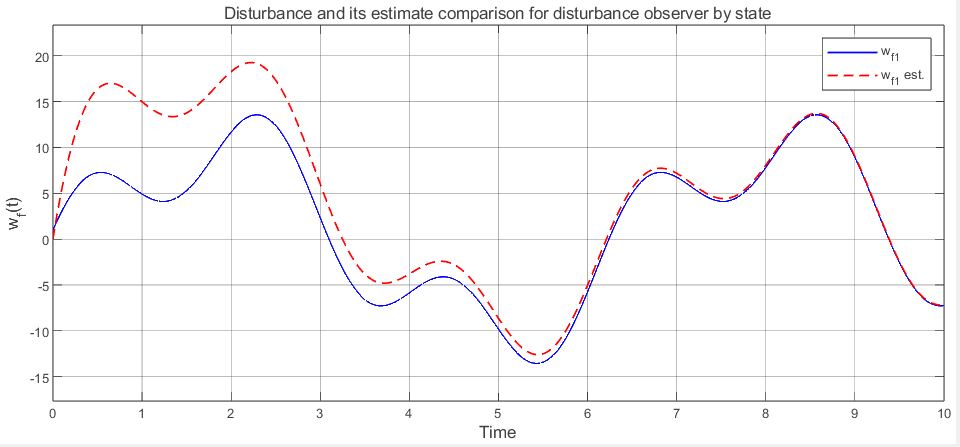
\includegraphics[scale=0.6]{3task_wfhwf1.png}
        \captionsetup{skip=0pt}
        \caption{График возмущения $w_{f_1}(t)$ и его оценки $\hat{w}_{f_1}(t)$ (набл. возм. по сост.)}
        \label{fig:3task_wfhwf1}
    \end{figure}
    \begin{figure}[H]
        \centering
        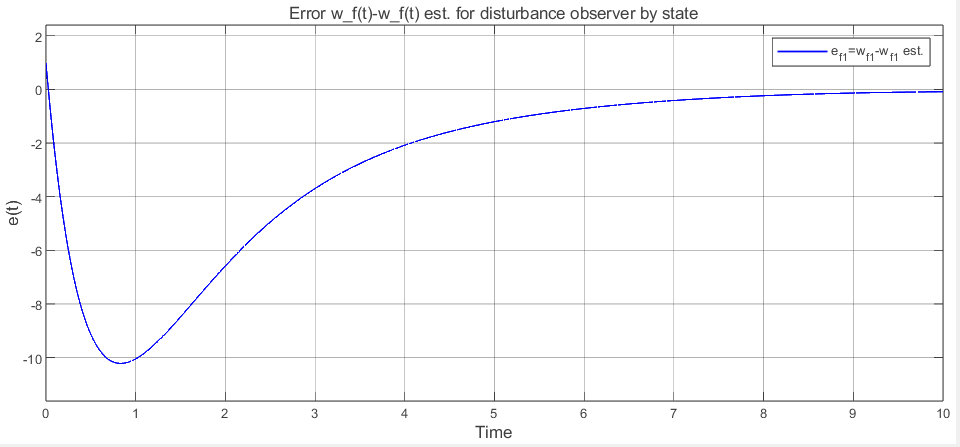
\includegraphics[scale=0.6]{3task_ef1.png}
        \captionsetup{skip=0pt}
        \caption{График ошибки $e_{f_1}(t)=w_{f_1}(t)-\hat{w}_{f_1}(t)$ (набл. возм. по сост.)}
        \label{fig:3task_ef1}
    \end{figure}
    \begin{figure}[H]
        \centering
        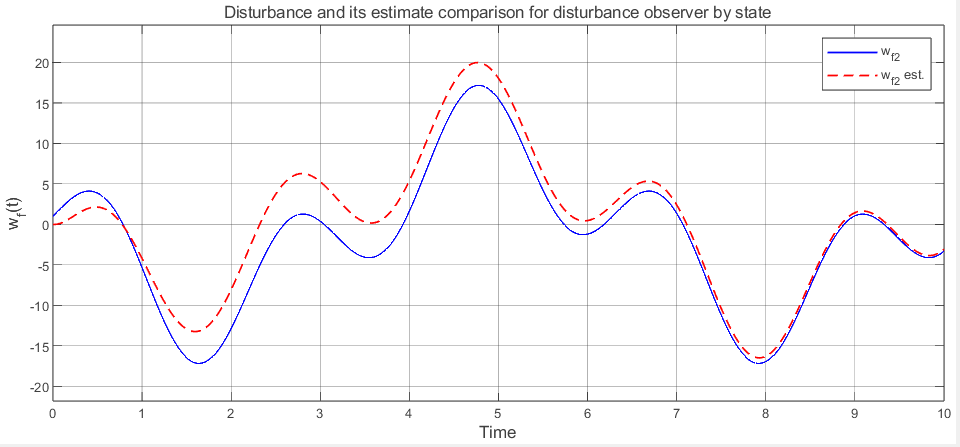
\includegraphics[scale=0.6]{3task_wfhwf2.png}
        \captionsetup{skip=0pt}
        \caption{График возмущения $w_{f_2}(t)$ и его оценки $\hat{w}_{f_2}(t)$ (набл. возм. по сост.)}
        \label{fig:3task_wfhwf2}
    \end{figure}
    \begin{figure}[H]
        \centering
        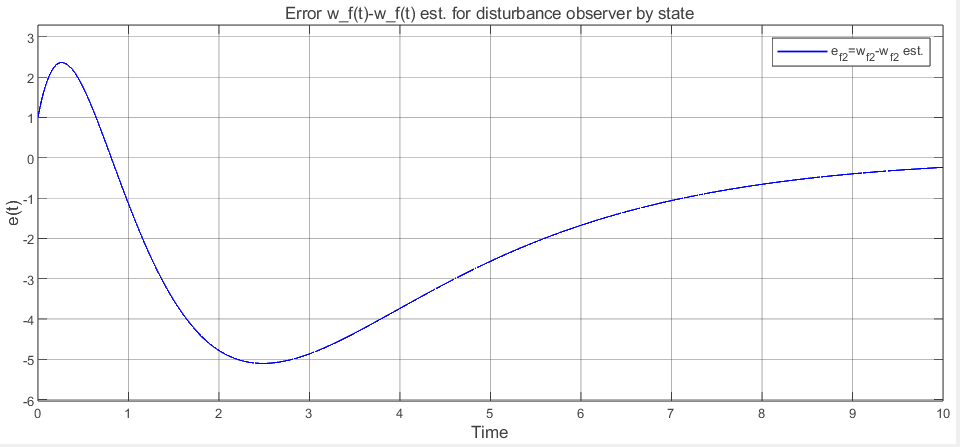
\includegraphics[scale=0.6]{3task_ef2.png}
        \captionsetup{skip=0pt}
        \caption{График ошибки $e_{f_2}(t)=w_{f_2}(t)-\hat{w}_{f_2}(t)$ (набл. возм. по сост.)}
        \label{fig:3task_ef2}
    \end{figure}
    \begin{figure}[H]
        \centering
        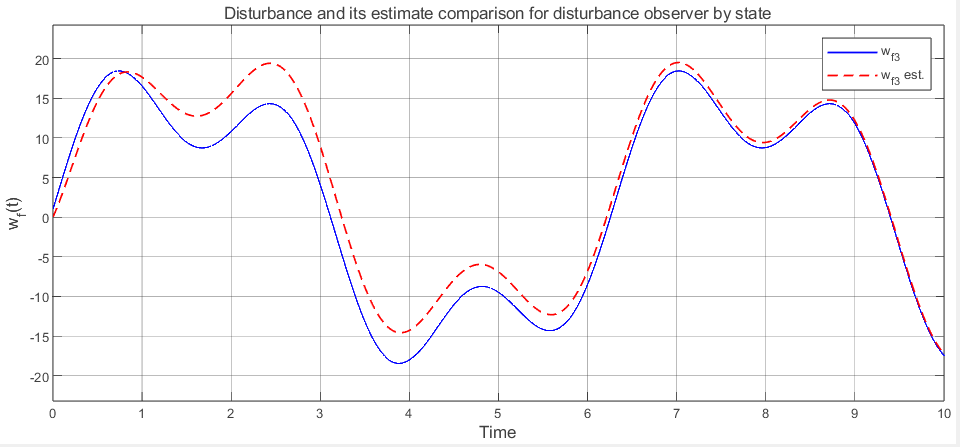
\includegraphics[scale=0.6]{3task_wfhwf3.png}
        \captionsetup{skip=0pt}
        \caption{График возмущения $w_{f_3}(t)$ и его оценки $\hat{w}_{f_3}(t)$ (набл. возм. по сост.)}
        \label{fig:3task_wfhwf3}
    \end{figure}
    \begin{figure}[H]
        \centering
        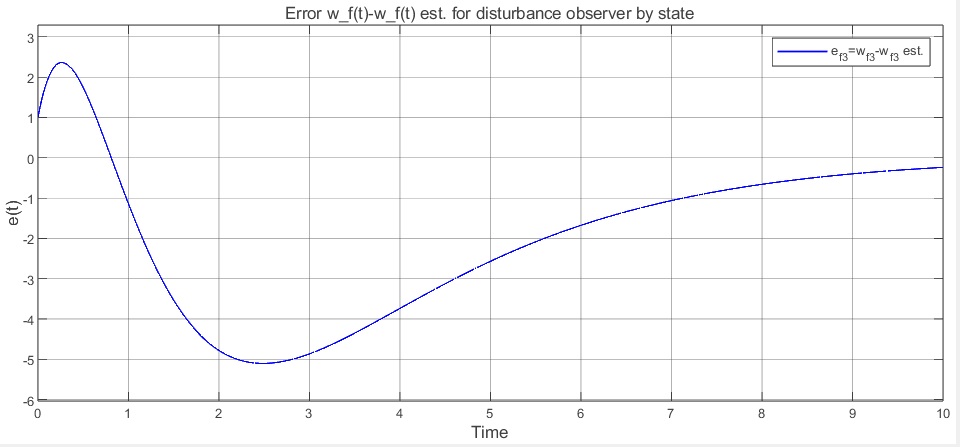
\includegraphics[scale=0.6]{3task_ef3.png}
        \captionsetup{skip=0pt}
        \caption{График ошибки $e_{f_3}(t)=w_{f_3}(t)-\hat{w}_{f_3}(t)$ (набл. возм. по сост.)}
        \label{fig:3task_ef3}
    \end{figure}
    \begin{figure}[H]
        \centering
        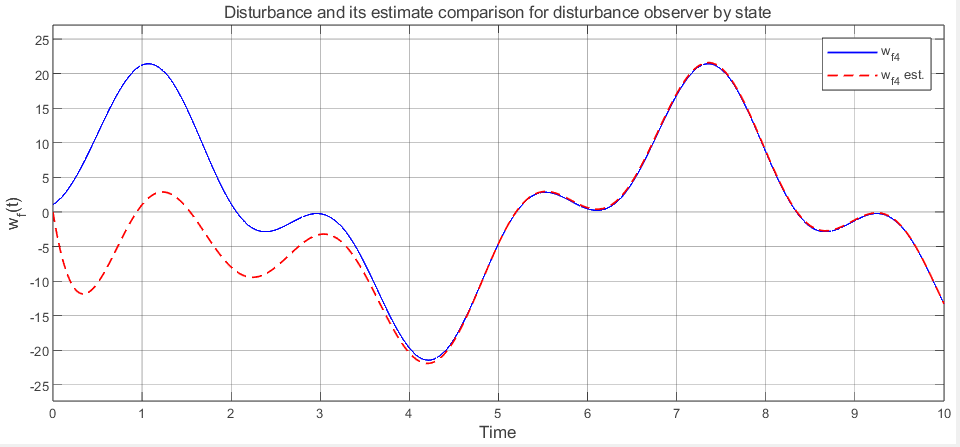
\includegraphics[scale=0.6]{3task_wfhwf4.png}
        \captionsetup{skip=0pt}
        \caption{График возмущения $w_{f_4}(t)$ и его оценки $\hat{w}_{f_4}(t)$ (набл. возм. по сост.)}
        \label{fig:3task_wfhwf4}
    \end{figure}
    \begin{figure}[H]
        \centering
        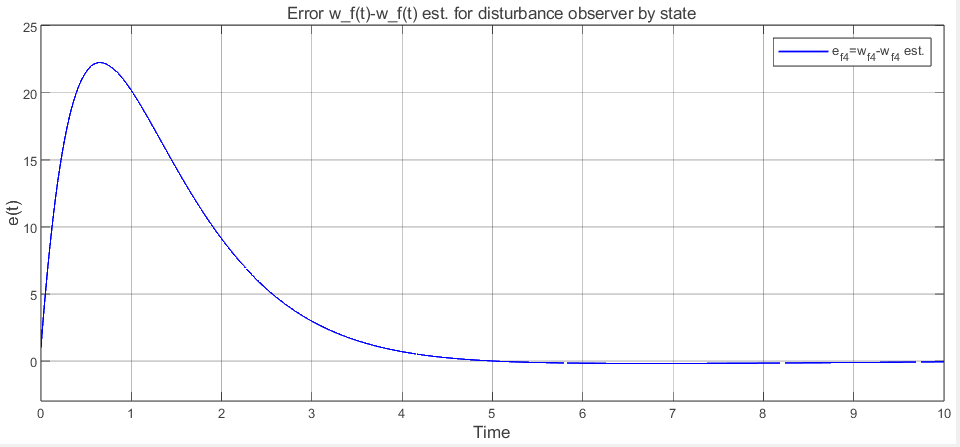
\includegraphics[scale=0.6]{3task_ef4.png}
        \captionsetup{skip=0pt}
        \caption{График ошибки $e_{f_4}(t)=w_{f_4}(t)-\hat{w}_{f_4}(t)$ (набл. возм. по сост.)}
        \label{fig:3task_ef4}
    \end{figure}
    \begin{figure}[H]
        \centering
        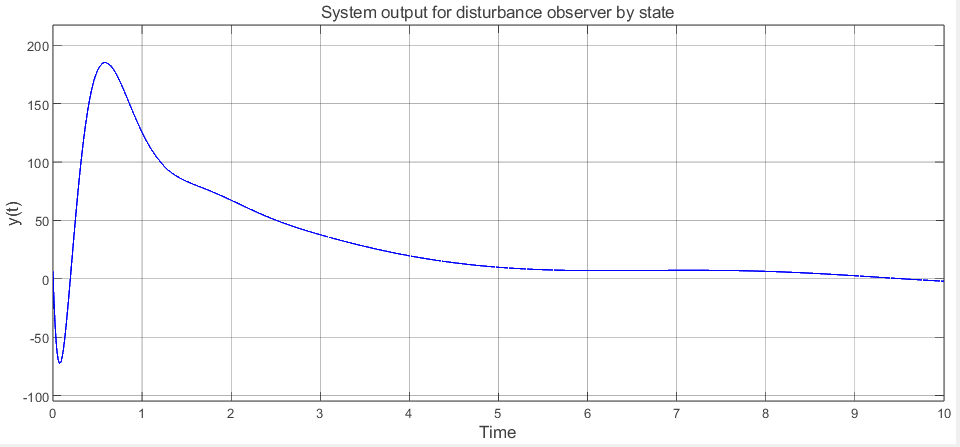
\includegraphics[scale=0.6]{3task_y1.png}
        \captionsetup{skip=0pt}
        \caption{График выхода системы $y(t)$ (набл. возм. по сост.)}
        \label{fig:3task_y1}
    \end{figure}
    \begin{figure}[H]
        \centering
        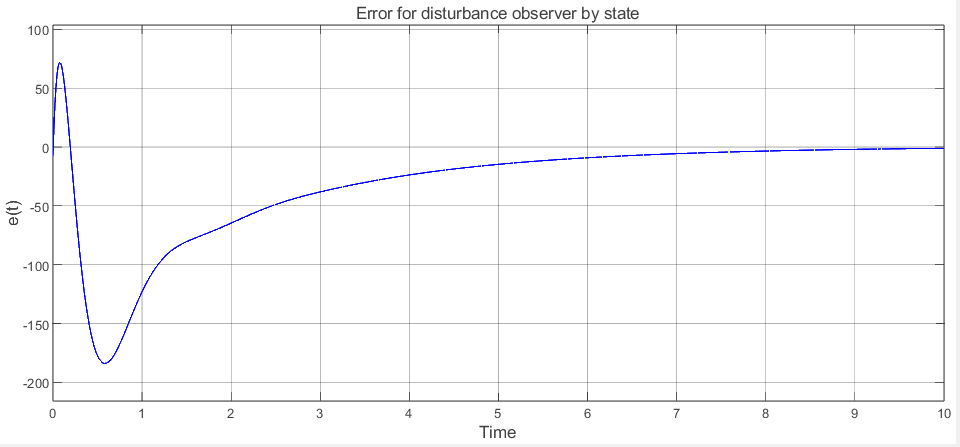
\includegraphics[scale=0.6]{3task_ey1.png}
        \captionsetup{skip=0pt}
        \caption{График ошибки $e(t)=g(t)-y(t)$ (набл. возм. по сост.)}
        \label{fig:3task_ey1}
    \end{figure}


    \subsection{Наблюдатель возмущения по выходу}
    Наблюдатель возмущения (работает при ненулевой $D_f$)
    $$
    \begin{cases}
        \hat{f}=D_ff=y-Cx-Du,\\
        \dot{\bar{w}}=\Gamma\bar{w}_f+Y\hat{f},\\
        \hat{w}_f=Q^{-1}\bar{w}_f;
    \end{cases}
    $$
    Цель остается такой же. Зададим желаемую динамику наблюдателя $\left( \Gamma,Y \right)$
    $$
    \Gamma=\begin{bmatrix}
        -0.5 &0 &0 &0\\
        0 &-1 &0 &0\\
        0 &0 &-1.5 &0\\
        0 &0 &0 &-2
    \end{bmatrix},\ Y=\begin{bmatrix}
        1\\1\\1\\1
    \end{bmatrix};
    $$
    Остается решить уравнение типа Сильвестра относительно $Q_{out}$
    $$
    Q_{out}\Gamma_f-\Gamma Q_{out}=YD_fY_f
    $$
    Получаем
    $$
    Q_{out}=\begin{bmatrix}
    -84.1514  &-29.1243   &70.2270  &-41.9135\\
  -46.6000  &-17.6000   &40.0000  &-23.0000\\
  -25.6000  &-10.6462   &22.6462  &-12.4000\\
  -15.1077   &-6.9231   &13.7846   &-7.0923
    \end{bmatrix},
    $$
    $$
    Q^{-1}=\begin{bmatrix}
        -4.1094   &15.7648  &-19.2273    &6.7770\\
   -7.1320   &34.6518  &-56.9446   &29.3341\\
   -9.4484   &43.5559  &-68.5269   &34.3983\\
   -2.6486   &17.2489  &-36.6460   &23.6454
    \end{bmatrix};
    $$


    \subsection{Схема моделирования системы с наблюдателем возмущения по
    выходу. Компьютерное моделирование системы}
    Построим схему и выполним компьютерное моделирование
    \begin{figure}[H]
        \centering
        \includegraphics[scale=0.5]{3task_scheme_2.png}
        \captionsetup{skip=0pt}
        \caption{Схема моделирования системы с наблюдателем возмущения по выходу}
        \label{fig:3task_scheme_2}
    \end{figure}
    \begin{figure}[H]
        \centering
        \includegraphics[scale=0.6]{3task_u2.png}
        \captionsetup{skip=0pt}
        \caption{График управления $u(t)$ (набл. возм. по вых.)}
        \label{fig:3task_u2}
    \end{figure}
    \begin{figure}[H]
        \centering
        \includegraphics[scale=0.6]{3task_x2.png}
        \captionsetup{skip=0pt}
        \caption{График вектора сост. ОУ $x(t)$ с наблюдателем возмущения по выходу}
        \label{fig:3task_x2}
    \end{figure}
    \begin{figure}[H]
        \centering
        \includegraphics[scale=0.6]{3task_wfhwf12.png}
        \captionsetup{skip=0pt}
        \caption{График возмущения $w_{f_1}(t)$ и его оценки $\hat{w}_{f_1}(t)$ (набл. возм. по вых.)}
        \label{fig:3task_wfhwf12}
    \end{figure}
    \begin{figure}[H]
        \centering
        \includegraphics[scale=0.6]{3task_ef12.png}
        \captionsetup{skip=0pt}
        \caption{График ошибки $e_{f_1}(t)=w_{f_1}(t)-\hat{w}_{f_1}(t)$ (набл. возм. по вых.)}
        \label{fig:3task_ef12}
    \end{figure}
    \begin{figure}[H]
        \centering
        \includegraphics[scale=0.6]{3task_wfhwf22.png}
        \captionsetup{skip=0pt}
        \caption{График возмущения $w_{f_2}(t)$ и его оценки $\hat{w}_{f_2}(t)$ (набл. возм. по вых.)}
        \label{fig:3task_wfhwf22}
    \end{figure}
    \begin{figure}[H]
        \centering
        \includegraphics[scale=0.6]{3task_ef22.png}
        \captionsetup{skip=0pt}
        \caption{График ошибки $e_{f_2}(t)=w_{f_2}(t)-\hat{w}_{f_2}(t)$ (набл. возм. по вых.)}
        \label{fig:3task_ef22}
    \end{figure}
    \begin{figure}[H]
        \centering
        \includegraphics[scale=0.6]{3task_wfhwf32.png}
        \captionsetup{skip=0pt}
        \caption{График возмущения $w_{f_3}(t)$ и его оценки $\hat{w}_{f_3}(t)$ (набл. возм. по вых.)}
        \label{fig:3task_wfhwf32}
    \end{figure}
    \begin{figure}[H]
        \centering
        \includegraphics[scale=0.6]{3task_ef32.png}
        \captionsetup{skip=0pt}
        \caption{График ошибки $e_{f_3}(t)=w_{f_3}(t)-\hat{w}_{f_3}(t)$ (набл. возм. по вых.)}
        \label{fig:3task_ef32}
    \end{figure}
    \begin{figure}[H]
        \centering
        \includegraphics[scale=0.6]{3task_wfhwf42.png}
        \captionsetup{skip=0pt}
        \caption{График возмущения $w_{f_4}(t)$ и его оценки $\hat{w}_{f_4}(t)$ (набл. возм. по вых.)}
        \label{fig:3task_wfhwf42}
    \end{figure}
    \begin{figure}[H]
        \centering
        \includegraphics[scale=0.6]{3task_ef42.png}
        \captionsetup{skip=0pt}
        \caption{График ошибки $e_{f_4}(t)=w_{f_4}(t)-\hat{w}_{f_4}(t)$ (набл. возм. по вых.)}
        \label{fig:3task_ef42}
    \end{figure}
    \begin{figure}[H]
        \centering
        \includegraphics[scale=0.6]{3task_y2.png}
        \captionsetup{skip=0pt}
        \caption{График выхода системы $y(t)$ (набл. возм. по вых.)}
        \label{fig:3task_y2}
    \end{figure}
    \begin{figure}[H]
        \centering
        \includegraphics[scale=0.6]{3task_ey2.png}
        \captionsetup{skip=0pt}
        \caption{График ошибки $e(t)=g(t)-y(t)$ (набл. возм. по вых.)}
        \label{fig:3task_ey2}
    \end{figure}


    \subsection{Сравнение результатов}
    При наблюдателе возмущения по состоянию $\hat{w}_f(t)$
    быстрее сходится к $w_f(t)$, чем при набл. возм. по выходу.
    При наблюдаетеле возмущения по выходу в целом ошибки $e_f(t)$
    сравнительно больше, выход системы $y(t)$ имеет несколько больше осцилляций.
    В обоих способах задания 3 выход системы имеет
    меньшую амплитуду в сравнении с заданием 2. В общем во всех методах
    поведения систем схожи.


    \section{Общий вывод по работе}
    В данной лабораторной работе были рассмотрены матричные
    уравнения Франкиса-Дэвисона и различные наблюдатели,
    такие как расширенный задающего воздействия, редуцированный возмущения по состоянию,
    редуцированный возмущения по выходу. В каждом случае были проведены
    расчеты и компьютерное моделирование. Результаты подтверждают
    корректность расчетов и рассуждений. Результаты были сравнены.


    \section{Приложение А}
    \begin{lstlisting}[label=task1, caption={Программа для задания 1}]
    % plant parameters
    A=[5 2 7;
       2 1 2;
      -2 -3 -4];
    B=[3;1;-1];
    Bf=[-4 -1;
        0 0;
        4 0];
    C=[2 0 3];
    D=2;
    Df=[8 3];

    Gf=[25 6 -20 11;
        14 3 -10 4;
        40 11 -31 17;
        6 4 -4 3];
    Yf=[8 2 -6 4;
    -20 -6 16 -9];

    Gg = [0 1 0;
         -1 0 0;
          0 0 0];
    Yg=[4 0 -1];
    wg0 = [0;1;1];

    % A eigenvalues
    A_eig = eig(A)

    % Jordan matrix
    [P1, J] = jordan(A);
    Pjre(:,1) = P1(:,1);
    Pjre(:,2) = imag(P1(:,2));
    Pjre(:,3) = real(P1(:,3))
    Pjre_inv = Pjre^-1
    Aj_re = Pjre_inv * A * Pjre
    B_jre = Pjre_inv * B

    % G eigenvalues
    Gf_eig = eig(Gf)
    Gg_eig = eig(Gg)

    % solving Riccati: feedback comp
    Q = eye(3);
    v = 2;
    R = 1;
    a = 2;

    Aa = A + eye(3) * (a-0.00000000000001);
    [Pk,K,e]=icare(Aa,sqrt(v)*B,Q,R);
    K=-inv(R)*B'*Pk
    eK=eig(A+B*K)

    % check Frankis-Davison: Kg
    Gg_eig(1)
    check_Kg1 = [(A+B*K)-eye(3)*Gg_eig(1) B; (C+D*K) D]
    rank(check_Kg1)

    Gg_eig(2)
    check_Kg2 = [(A+B*K)-eye(3)*Gg_eig(2) B; (C+D*K) D]
    rank(check_Kg2)

    Gg_eig(3)
    check_Kg3 = [(A+B*K)-eye(3)*Gg_eig(3) B; (C+D*K) D]
    rank(check_Kg3)

    % solving Frankis-Davison: Kg
    cvx_begin sdp
    variable Pg(3,3)
    variable Kg(1,3)
    Pg*Gg-(A+B*K)*Pg == B*Kg;
    (C+D*K)*Pg+D*Kg == Yg;
    cvx_end

    Pg=Pg
    Kg=Kg

    % check Frankis-Davison: Kf
    Gf_eig(1)
    check_Kf1 = [(A+B*K)-eye(3)*Gf_eig(1) B; (C+D*K) D]
    rank(check_Kf1)

    Gf_eig(2)
    check_Kf2 = [(A+B*K)-eye(3)*Gf_eig(2) B; (C+D*K) D]
    rank(check_Kf2)

    Gf_eig(3)
    check_Kf3 = [(A+B*K)-eye(3)*Gf_eig(3) B; (C+D*K) D]
    rank(check_Kf3)

    Gf_eig(4)
    check_Kf4 = [(A+B*K)-eye(3)*Gf_eig(4) B; (C+D*K) D]
    rank(check_Kf4)

    % solving Frankis-Davison: Kf
    cvx_begin sdp
    variable Pf(3,4)
    variable Kf(1,4)
    Pf*Gf-(A+B*K)*Pf-Bf*Yf == B*Kf;
    (C+D*K)*Pf+D*Kf == -Df*Yf;
    cvx_end

    Pf=Pf
    Kf=Kf
    \end{lstlisting}


    \section{Приложение Б}
    \begin{lstlisting}[label=task2, caption={Программа для задания 2}]
    % plant parameters
    A=[5 2 7;
       2 1 2;
      -2 -3 -4];
    B=[3;1;-1];
    Bf=[-4 -1;
        0 0;
        4 0];
    C=[2 0 3];
    D=2;
    Df=[8 3];

    Gf=[25 6 -20 11;
        14 3 -10 4;
        40 11 -31 17;
        6 4 -4 3];
    Yf=[8 2 -6 4;
    -20 -6 16 -9];

    Gg = [0 1 0;
         -1 0 0;
          0 0 0];
    Yg=[4 0 -1];
    wg0 = [0;1;1];

    K=[2.1111 -13.4448 1.6787];
    Kg=[-0.0932 18.6951 -8.1152];
    Kf=[-725.9021 -225.1491 586.1685 -359.3897];

    G=[-1 0 0;
        0 -5 0;
        0 0 -10];
    Y=[1; 1; 1];

    % find Q
    cvx_begin sdp
    variable Q(3,3)
    Q*Gg-G*Q == Y*Yg;
    cvx_end

    Q=Q
    invQ=inv(Q)

    null1=[0 0 0;
           0 0 0;
           0 0 0;
           0 0 0];
    null2=[0;0;0;0];
    barA = [Gf null1;
            Bf*Yf A]
    barB = [null2;B]
    barC=[Df*Yf C]

    % solving Riccati
    QL = eye(7);
    v = 1;
    R = 1;

    [P,L,e]=icare(barA',barC',QL,R);
    L=-P*barC'*R^-1
    \end{lstlisting}


    \section{Приложение В}
    \begin{lstlisting}[label=task3,caption={Программа для задания 3}]
    % plant parameters
    A=[5 2 7;
       2 1 2;
      -2 -3 -4];
    B=[3;1;-1];
    Bf=[-4 -1;
        0 0;
        4 0];
    C=[2 0 3];
    D=2;
    Df=[8 3];

    Gf=[25 6 -20 11;
        14 3 -10 4;
        40 11 -31 17;
        6 4 -4 3];
    Yf=[8 2 -6 4;
    -20 -6 16 -9];

    Gg = [0 1 0;
         -1 0 0;
          0 0 0];
    Yg=[4 0 -1];
    wg0 = [0;1;1];

    K=[2.1111 -13.4448 1.6787];
    Kg=[-0.0932 18.6951 -8.1152];
    Kf=[-725.9021 -225.1491 586.1685 -359.3897];
    Q =[2.0000 -2.0000 -1.0000;
        0.7692 -0.1538 -0.2000;
        0.3960 -0.0396 -0.1000];
    invQ=inv(Q)

    G=[-0.5 0 0 0;
        0 -1 0 0;
        0 0 -1.5 0;
        0 0 0 -2];
    Y=[1 0 1 0;
       0 1 0 1];
    newY=[1;1;1;1];

    % find QL
    cvx_begin sdp
    variable QL(4,4)
    QL*G-Gf'*QL == Yf'*Y;
    cvx_end

    QL=QL
    L=-Y*QL^-1;
    L=L'

    % find barC
    cvx_begin sdp
    variable barC(2,3)
    barC*Bf == eye(2);
    cvx_end

    barC=barC

    F=Gf-L*Yf

    % find Qout
    cvx_begin sdp
    variable Qout(4,4)
    Qout*Gf-G*Qout == newY*Df*Yf;
    cvx_end

    Qout=Qout
    invQout=inv(Qout)
    \end{lstlisting}
\end{document}